\chapter{基于弱监督学习的深度级联显著性检测网络}
\renewcommand{\leftmark}{第二章\quad 基于弱监督学习的深度级联显著性检测网络}
\renewcommand{\figurename}{图}

\section{引言}
在前文的分析中,本文有提及现今基于深度网络视频显著性检测的方法所存在几个关键性问题,其中首先要解决的问题就是训练数据不足的问题。在前一章中,本文提到现有的数据集很少,而且为了验证提出的方法,不能把全部的数据都用于训练。而且,这些数据的像素级标签大多不连续,有些是每5帧记一个标签,如ViSal\cite{ViSalWang},有些是每20帧记一个标签,如FBMS\cite{ochs2013segmentation}。这些非连续的标记数据可以运用于测试,但是运用于训练则比较困难。因此,一些文献则设法通过其他方法来完成深度网络的训练。Wang等则在文献\cite{8047320}中提出使用光流模拟的方法,即使用其他有标定的图像数据集,在其中运用光流的原理,在图像上进行扰动,从而使静态图像的一些像素产生位移,进而有运动的效果,而且像素级标签也可以这样模拟,这样可以得到足够的模拟数据。本文则从弱监督学习方向考虑解决数据不足问题,在网络训练中自动地生成弱标签,并依靠显著图融合的方法不断地增强生成的弱标签,从而辅助深度网络学习。并且,考虑到运动特征不鲁棒,本文考虑从网络外部引入一个运动先验,并结合网络中产生的静态先验共同引导深度网络产生准确的显著图。

本章的内容组织由四个部分组成。首先是引言,介绍所提出方法的动机。其次是详细的方法描述,其包括四个模块:级联深度网络的总体结构、运动先验的提取、弱监督学习算法、像素级显著图精炼。接着是实验结果与详细的分析。最后则是对此方法的总结。

\begin{figure*}
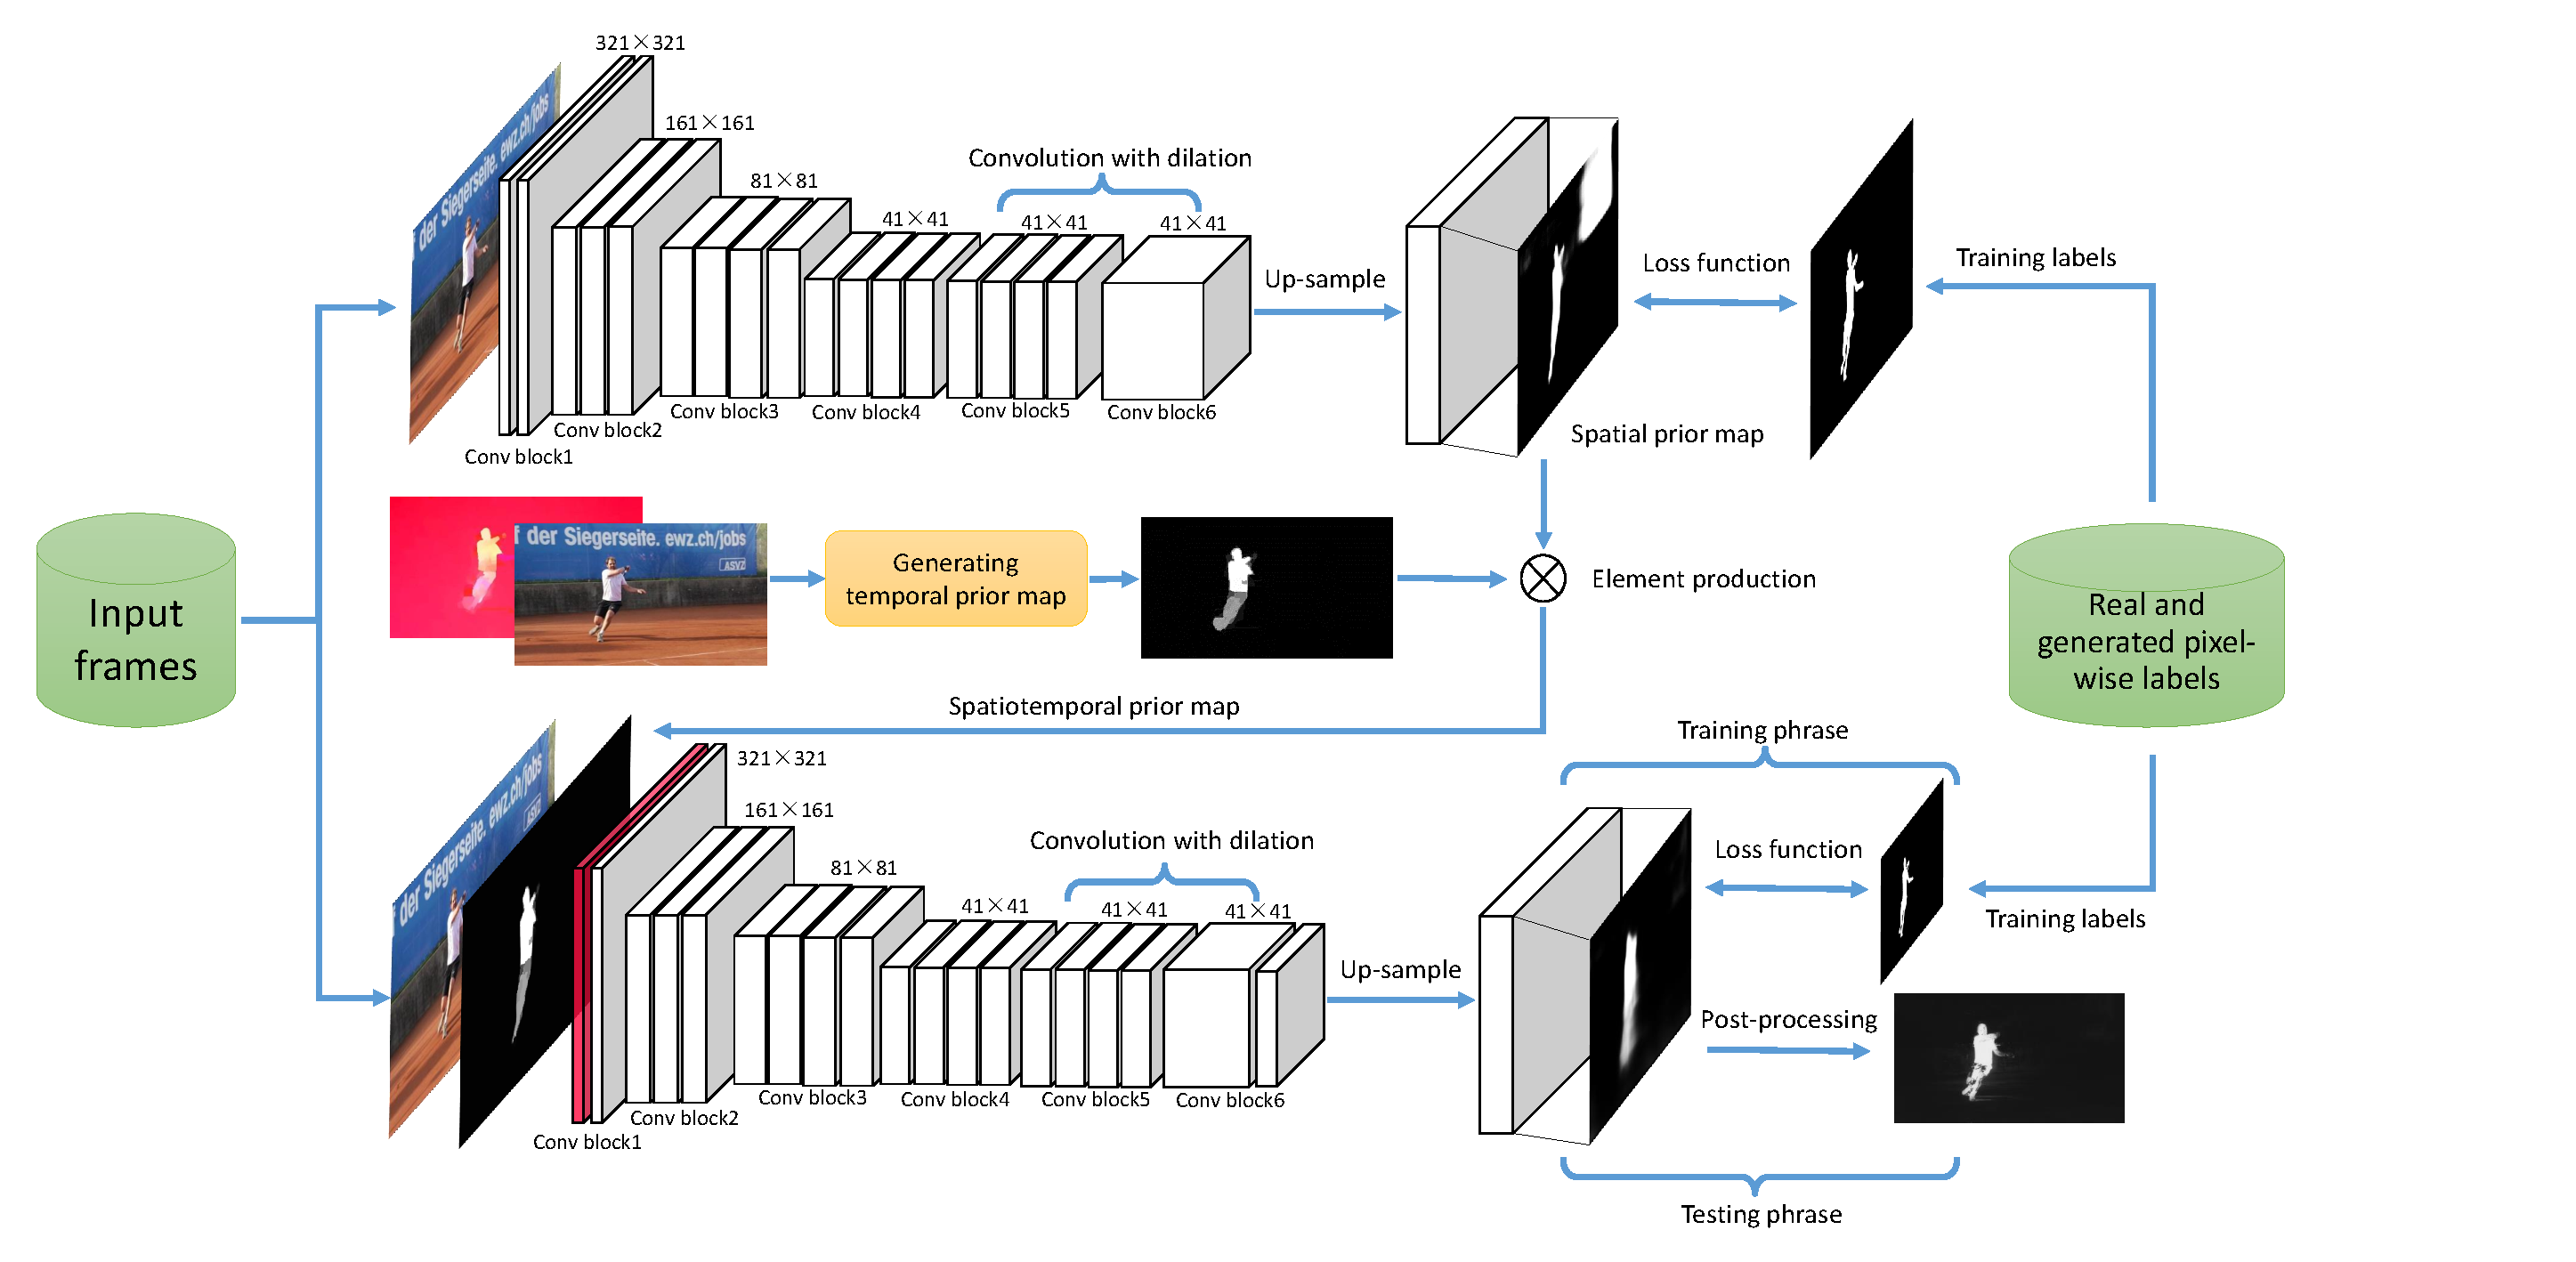
\includegraphics[width=15cm]{figures/scnn_framework}
\caption{级联深度的结构图}
\label{figure2}
\end{figure*}

\section{方法描述}
\subsection{级联深度网络结构}
本方法所提出的级联网络(SCNN)如图\ref{figure2}所示,输入一个视频帧在第一个子网中先生成静态先验图。另一个方面,运动先验则由光流图和视频帧共同生成。之后两个先验图则采用像素级相乘的方式进行融合,并把融合后的先验输入到第二个子网中去引导训练。最后,再使用一个稠密的条件随机场进行精炼,从而生成最终的显著图。

SCNN是有两个相同结构的VGG网络级联而成。相对于原有的由五个卷积块组成的VGG,SCNN中的VGG有所修改,为了生成检测图,VGG最后的两个全连接层对应转化为卷积层。同时,为了恢复原有的尺度,在网络的最上层加入的线性上采样层。在SCNN中,每一个卷积操作可以表述为:
\begin{equation}
 \label{eq1}
   f(X; W,b) = \sigma (W * X + b)
\end{equation}

其中,$f(\cdot)$表示通过卷积操作生成的特征图;$X$表示输入三通道的视频帧($X \in R^{h*w*c}$);$b$ 为偏置项; $W$是卷积参数; $\sigma(\cdot)$ 表示的是ReLU激活函数。

原始的VGG网络是包括五个下采样层,每一层可以把特征图缩小两倍,从而更好地提取语义信息。然而,在显著性检测中,下采用越多越不利于恢复整体图像的上下文信息。为了保证空间上下文信息,原始的基于VGG的FCN网络\cite{simonyan2014very},在网络的第一个卷积层加入100个像素值为0的padding,从而增加输入图像的尺寸。但是,这种方法也增加了许多冗余的像素,从而直接影响网络的学习。在SCNN中,采取了减小下采样的方式,最后的两个最大池化层被移除,从而保证特征图的尺度。而且,为了保证有足够大的感受野,膨胀卷积\cite{chen2014semantic}则被引入。

在SCNN中,多尺度的特征图也充分被使用。而且,不像文献\cite{li2016deep}把所有的卷积块后都设置了上采样层来提取特征。本文通过实验分析,前四个卷积块上采样的特征图对最终的显著图影响较小。所以,为了简化网络和提高计算效率,SCNN只利用了最后两个卷积块的尺度信息,利用上采样层恢复尺寸后,使用线性相加的方式进行多尺度特征融合。

由于运动特征不好用静态的网络提取,本文采用外部引入运动特征的方法。由光流和视频帧产生运动先验会与级联网络第一个子网生成的静态先验融合成时空先验,从而引导第二个子网进行学习。由于时空先验的嵌入,SCNN中第二个子网的卷积操作可以改写为:

\begin{equation}
\label{eq2}
\begin{aligned}
   f(X, P; W_1, W_2,b) &= \sigma (W_1 * X + W_2 * P + b) \\
                        &= \sigma([W_1 \  W_2]*[X \  P]^T  + b)
\end{aligned}
\end{equation}

其中, $P$ 表示时空先验图; $W_1$是针对输入帧 $X$的卷积参数;$W_2$是针对有时空先验图$P$的卷积参数;$b$是偏置项。

为了更新优化整个SCNN网络,在网络的末端需要设置一个损失函数来计算生成的显著图$S \in [0,1]^{h*w*1}$与真值$G \in [0,1]^{h*w*1}$的误差,其中$h$与$w$分别为输入视频帧的高与宽。同时,考虑到像素级分类中的标签不平衡,本文引入了加权交叉熵的损失函数:
\begin{equation}
 \label{eq3}
 \begin{aligned}
   L(S, G) = &-\alpha \sum^{h*w}_{i=1} g_i \log P(s_i = 1|X_i, W) \\
             &- (1 - \alpha) \sum^{h*w}_{i=1} (1-g_i)\log P(s_i = 0|X_i, W)
   \end{aligned}
\end{equation}

$s_i \in S$ and $ g_i \in G$分别表示像素的显著值和真值;$\alpha$表示的是平衡因子,其值是背景像素与所有像素的比值。

\subsection{运动先验的提取}
为了是网络具备足够的运动特性,SCNN引入了一个有静态先验图$P_s$与运动先验图$P_t$组成的时空先验图$P$,从而引导级联网络学习显著性特征。既然是先验图,保持准确率要比召回率要重要,本文不期望时空先验图可以高亮出完整的显著性目标,但是至少保证高亮出的区域是可靠的。因此,本文使用的是像素级相乘来融合静态和运动先验图:
\begin{equation}
 \label{eq3_3}
 \begin{aligned}
   P = P_s \otimes P_t
   \end{aligned}
\end{equation}

其中,$\otimes$表示的是像素相乘操作。这一操作可以高亮出静态与运动先验图中共享的部分和抑制那些只存在一个先验图中的噪声区域。

在上一小节中,静态先验是有级联网络中第一个全卷积子网生成的。具体是这个子网把视频帧作为输入,从而相应的特征图。然后,在网络的最后一层使用sigmoid激活函数,从而生成静态先验,其过程可以表示为:
\begin{equation}
 \label{eq3_1}
 \begin{aligned}
   P_s = \Psi\bigg(U_{s}\big(F_{s}(X;\theta)\big)\bigg)
   \end{aligned}
\end{equation}

$\Psi(\cdot)$表示sigmoid激活;$U_{s}(\cdot)$则为上采样操作;$F_ {s}(\cdot)$表示卷积操作;$\theta$为网络的学习参数。在本文的实验中,线性上采样被用来保证静态先验图的尺寸与输入图像一致。

\begin{figure*}[tbp]
\center
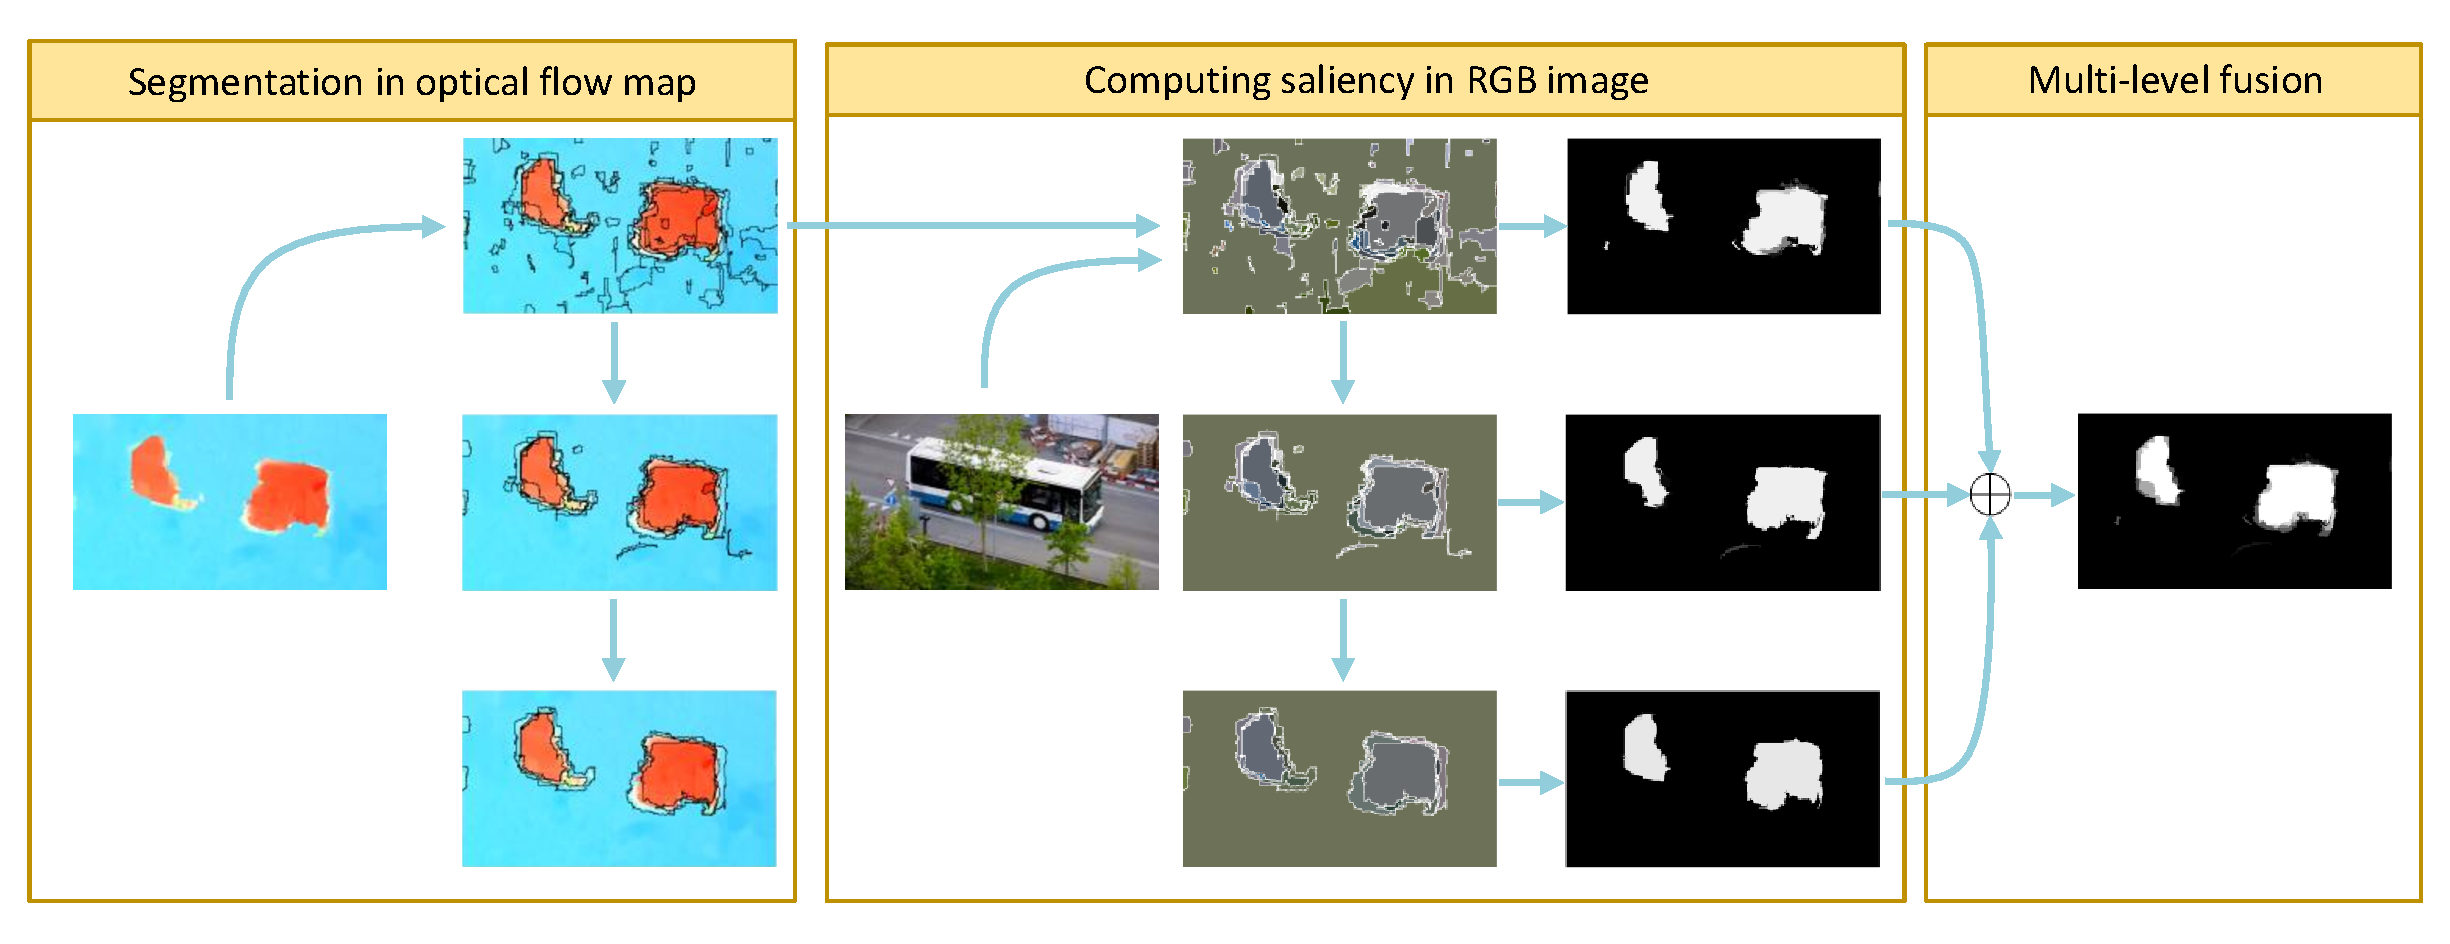
\includegraphics[width=15cm]{figures/segment}
\caption{运动先验生成流程图}
\label{temporal_prior}
\end{figure*}

为了生成优质的运动先验图$P_t$,本文提出了一个新颖地利用光流图提取的方法。具体的流程图如图\ref{temporal_prior},首先,本文先利用基于图分割的方法,采用不同的分割参数对光流图分割$M$次,从而得到$M$个分割图像。然后,再那到超像素区域$r_i^j (j= 1, 2,..., M)$(其中,$i$是超像素标识,$j$表示属于哪个分割图)后,在原来的RGB图像中提取图像块,并在填充成patch后输入AlexNet中提取深度特征。最后利用一个三层全连接的分类器来判断这个超像素是否显著。这一个过程可以总结为下面一个公式:
\begin{equation}
 \label{eq3_2}
 \begin{aligned}
   P_t(r_i)  = \frac{1}{M} \sum_{j=1}^M S^j\big(D(r_i^j)\big)
 \end{aligned}
\end{equation}

其中$D(\cdot)$表示对应超像素$r_i^j$的深度特征;$S^j(\cdot)$表示被分类器预测的显著概。在本文的实验室,为了包括效率,$M$设置为3。
\subsection{弱监督学习算法}

深度学习已经在计算机视觉的各个领域上都取得了很大的成成功。然而,其为数据驱动的方法,需要大量的训练数据来完成网络训练。在视频显著性检测任务中,虽然视频数据容易获取,但是与之对应的像素级标签需要大量的人工和时间来标定,这也是目前许多视频显著性检测的数据不能标定连续帧标签的原因。为了有足够的训练数据进行网络训练,文本提出了一种新颖的弱监督学习的方法来优化神经网络。本文先假设在训练过程中产生弱标签,并在训练中逐渐增强这些弱标签,这样这些标签应该可以对网络训练有帮助。因此,本文使用融合显著图的方法产生弱标签,并引入一种迭代训练的方法来完成弱监督网络学习。

\begin{figure*}[tbp]
 \centering
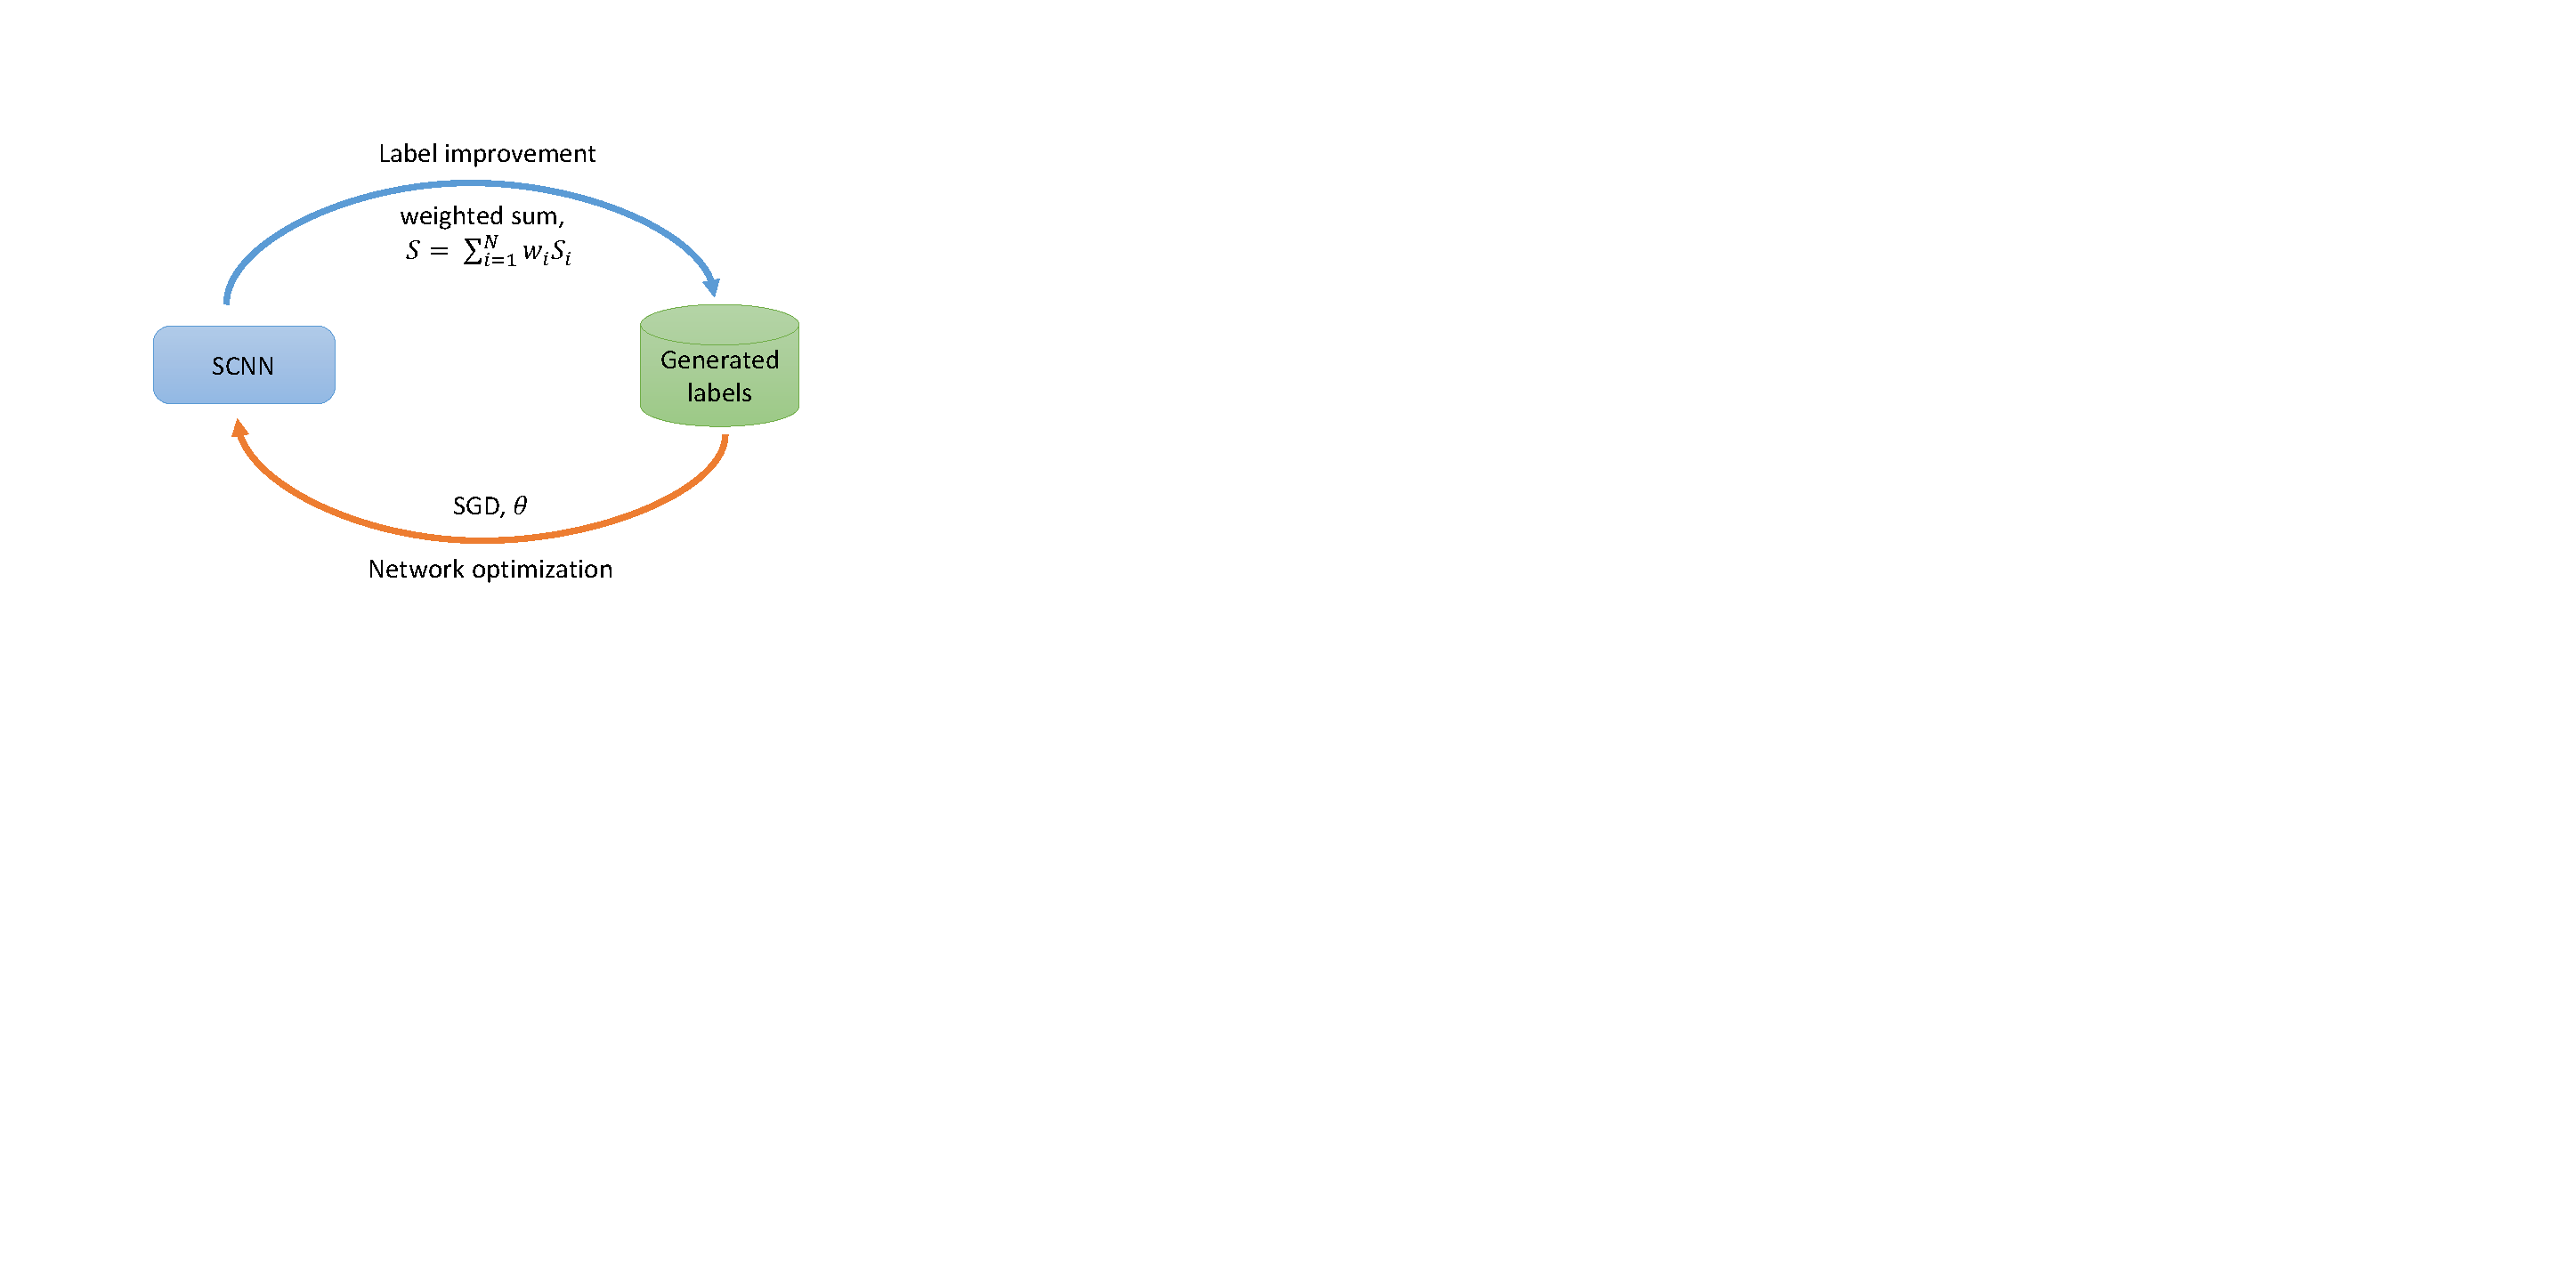
\includegraphics[width=10cm]{figures/labeling}
\caption{弱监督的方法产生标签并相互迭代的方法训练神经网络}
\label{weak_lables}
\end{figure*}

如图\ref{weak_lables}所示,本文提出的所监督学习方法包括两个部分:SCNN的网络训练和弱标签的提升。首先,给定标定数据,神经网络可利用随机梯度下降法进行网络训练,进而生成初步的显著图。然后,这些显著图与其静态显著性方法生成的显著图融合生成弱标签。接着,在网络训练过程中,交替迭代这两个过程,直到网络收敛。

在本文提出的弱监督训练方法中,融合显著性图的方法采用的是线性加权融合,可表示为:
\begin{equation}
S = \sum_{i=1}^{N} w_i * S_i
\label{eq4}
\end{equation}

其中$S_i (i = 1,\cdots,N )$表示的是SCNN和其他显著性检测方法生成的显著图,$N$为方法的个数。权重$\{w_1, w_2, ..., w_N\}$采用的最小二乘法进行求解:
\begin{equation}
w^* = \arg\min_{w_i} ||G - \sum_{i=1}^{N} w_i * S_i||
\label{eq5}
\end{equation}

$G$表示已经手工标定后的标签;$w^*$则为最优的权重。整个训练过程即为通过公式\ref{eq5},利用带标签的数据训练融合权重,再利用这些权重来融合特征图,最后得到弱标签。SCNN整个弱监督训练过程可以由算法\ref{alg1}描述。这些融合的显著图只会使用在训练阶段,在测试式,所有的显著性结果都会直接由SCNN生产。

本文实现时,融合的由静态显著图分别来自DCL\cite{li2016deep},RFCN\cite{wang2016saliency},DS\cite{li2016deepsaliency}
这三个方法是当时最好静态方法,可以直接生产较为准确的静态显著图。虽然这几个方法在检测视频显著性目标时会有瑕疵,但是随着本文SCNN显著图的引入,再加上线性融合,几种显著图会相互弥补。因此,本文可以利用这些融合的弱标签完成SCNN的网络训练。

\begin{algorithm}[tbp]
\caption{并行迭代弱监督训练策略}
\renewcommand{\algorithmicrequire}{\textbf{输入:}}
\renewcommand{\algorithmicensure}{\textbf{输出:}}

\newcommand\algorithmicestep{\textbf{网络优化:}}
\newcommand\ESTEP{\item[\algorithmicestep]}
\newcommand\algorithmicmstep{\textbf{弱标签增强:}}
\newcommand\MSTEP{\item[\algorithmicmstep]}

\label{alg1}
\begin{algorithmic}[1]

\REQUIRE 初始化网络参数 $\theta_0$和网络输入 $X$;初始的弱像素级标签 $G_0$是采用加权融合显著图$S_i$而成,其中其中初始权值为$w_0$;训练次数为$\beta$;
\ENSURE 训练结束后的网络参数 $\theta_\beta$
\FOR{ $t = 1, 2, ..., \beta $}
\ESTEP
\STATE 使用弱标签$G_{t-1}$和输入的视频帧$X$通过公式\ref{eq3}计算网络的损失函数;
\STATE 用随机梯度下降法(SGD)优化网络参数$\theta_t$;
\MSTEP
\STATE 在原有的融合显著图中加入SCNN生成的显著图重新融合,并使用公式\ref{eq5}更新融合的权值$w_t$;
\STATE 通过公式\ref{eq4}得到融合显著图$S$ 后,再利用Otsu阈值算法把生成弱标签转化为用于网络训练的二值化图像 $G_{t}$。
\ENDFOR
\end{algorithmic}
\end{algorithm}

\subsection{像素级显著图精炼}

SCNN已经可以准确地检测显著性区域,但是有些生成的显著图仍有些粗糙,显著目标的边缘不够精细。因此,本文引入一个稠密条件随机场(Dense-CRF)的方法来精炼由SCNN生成的显著图。具体地,需要先定义的条件随机场能量函数来对应显著标签,然后最小化这个能量函数,从而得到最佳的显著图。根据文献\cite{krahenbuhl2011efficient},能量函数定义如下:

\begin{equation}
   \label{eq6}
   E(s_i, s_j) = -\sum_i \log\Theta(s_i) + \sum_{i,j} \varphi_{ij}(s_i, s_j)
\end{equation}

其中,$s_i $ 和 $s_j$对应的是显著图中不同的两个像素点。公式中的第一项是一元势函数,$\Theta(s_i)$表示的是$s_i $这点的显著值。第二项是二元势函数,其可以展开为:

\begin{equation}
 \label{eq7}
 \begin{aligned}
   \varphi_{ij}(s_i, s_j) = \mu(s_i, s_j)[\omega_1&*\exp(-\frac{||p_i-p_j||^2}{2\delta_\alpha^2}-\frac{||I_i-I_j||^2}{2\delta_\beta^2}) \\
   &+ \omega_2*\exp(-\frac{||p_i-p_j||^2}{2\delta_\gamma^2})]
  \end{aligned}
\end{equation}

当$s_i \neq s_j$时,$\mu_{ij}(s_i, s_j) = 1$,否则为0,公式\ref{eq7}中的,第一项为前景项,若前景中颜色相似像素被认定为同一标签,可以用来提升周围像素的显著值。第二项则是平滑项,其目的是消除细小的孤立背景区域。$p_i, p_j$则表示像素的坐标;$I_i, I_j$为像素强度;参数$\delta_\alpha, \delta_\beta$控制空间距离,而$\delta_\gamma$则决定强对比度,$\omega_1$ 和 $\omega_2$则是两个优化项的参数。

\section{实验结果和分析}
在这一小节中,本文首先介绍几个通用的视频检测数据集和评价标准。之后,介绍本文在实现算法时需要注意的细节。接着,展示本文的实验结果并与其他显著性检测方法进行对比,同时也分析SCNN中各个模块的有效性。最后,展示SCNN的效率。
\subsection{数据集}

在SCNN方法中,本文主要使用了四个数据集来验证方法,分别是MSRA10K\cite{Liu2011Learning},SegTrackV2\cite{li2013video},FBMS\cite{brox2010object},DAVIS\cite{perazzi2016benchmark}。

\textbf{MSRA10K}包含10000个图像,分别从人物、动物、植物、交通标志等不同的场景获取。这是图像检测性目标检测常用的数据集。

\textbf{SegTrackV2}包含14个视频序列共1066帧。每个序列大约有100帧,而且每一帧都有与之对应的像素级标签。

\textbf{FBMS}有59个视频序列共13960帧。这个数据被分为两个部分:训练集和测试集,前者包含29个视频序列,后者则有30个序列。FBMS虽然视频帧数充足,但是其像素级标签则是不连续的,比如在测试集视频总共7306帧,却只有720帧有对应的像素级标签。

\textbf{DAVIS}相对于上述几个数据而言,其数据很完整,总共50个视频序列3455帧,且每一帧都有对应的像素级标签。同时,DAVIS的视频场景也复杂多样,包括多目标、带遮挡、目标形变、运动模糊等场景,是一个非常具有挑战性的数据集。

在本文的实验中,SCNN使用MSRA10K、SegTrackV2和FBMS的训练集进行网络训练。在FBMS测试集和DAVIS中做测试。

\subsection{评价方法}
对于评价标准,本文采用标准的PR曲线(precision-recall curve)来验证提出的方法。在计算PR曲线时,每一张显著图首先被归一化到[0,255]。在这个范围内,每一个整数作为阈值产生一个二值蒙版来计算准确率和召回率。同时,平均绝对误差(mean absolute error)也被用于评价本文提出方法。平均绝对误差是计算显著图和真值的平均差值,可以定义为公式\ref{eq8},其中$p_i$表示单个像素;$S$ and $G$分别表示显著图和对应的真值。
\begin{equation}
 \label{eq8}
   MAE = \frac{1}{|S|} \sum_i |S(p_i) - G(p_i)|
\end{equation}

\subsection{实现细节}

SCNN主要由Caffe深度学习库\cite{jia2014caffe}及其MATLAB API实现。作为补充,MATLAB自带的深度学习工具包\cite{Palm2012Prediction}也有使用。

在网络训练时,本文首先利用在ImageNet \cite{Russakovsky2015ImageNet}训练完成的VGGNet \cite{szegedy2015going}来初始化网络。 其次,MSRA10K被用以微调(finetune)FCN网络。之后,把两个FCN网络级联在一起组成SCNN。在融合静态先验和运动先验后,把融合的时空先验也引入SCNN进行网络微调,也由于加入一个额外通道,SCNN第二个FCN的输入需要重新使用Xavier进行初始化。最后,通过本文提出的弱监督学习策略,SegTrackV2和FBMS的训练集则被用来第二次微调SCNN网络。在测试阶段,SCNN产生的显著图则使用Dense CRF方法进行精炼,从而得到最后的输出。

在整个训练阶段,随机梯度下降(SGD)优化算法被用来优化SCNN网络。两次微调的网络初始学习率分别为$10^{-2}$ 和 $10^{-10}$;权重衰减为0.005;学习动量为0.9。

\subsection{方法对比}

在此次实验中,本文同时比较了图像显著性方法和视频显著性方法。其中,视频显著性方法有ST算法(space-time saliency detection)\cite{zhou2014time}、CS算法(cluster-based co-saliency
method) \cite{fu2013cluster}、SS算法(segmenting saliency detection) \cite{rahtu2010segmenting}、CG算法(consistent gradient based saliency)\cite{wang2015consistent}和SA算法(saliency-aware method)\cite{wang2015saliency}。图像显著性方法则包括DCL算法(deep contrast learning)\cite{li2016deep}、RFCN算法(recurrent fully convolutional network)\cite{wang2016saliency}、DSMT算法(deep saliency multi-task)\cite{li2016deepsaliency}、LEGS算法(local estimation and global search)\cite{wang2015deep}、MDF算法(visual saliency on multi-scale deep features)\cite{li2016visual}、Amulet算法(aggregating multi-level convolutional features)\cite{Zhang_2017_ICCV_Amulet}、WSS算法(saliency detection with image-level supervision)\cite{Wang2017Learning}、UCF算法(learning uncertain convolutional features)\cite{Zhang_2017_ICCV_UCF},同时还有两个非深度学习算法:SO算法(robust background detection)\cite{zhu2014saliency}和SF算法(saliency filters)\cite{perazzi2012saliency}。

\begin{figure*}[tbp]
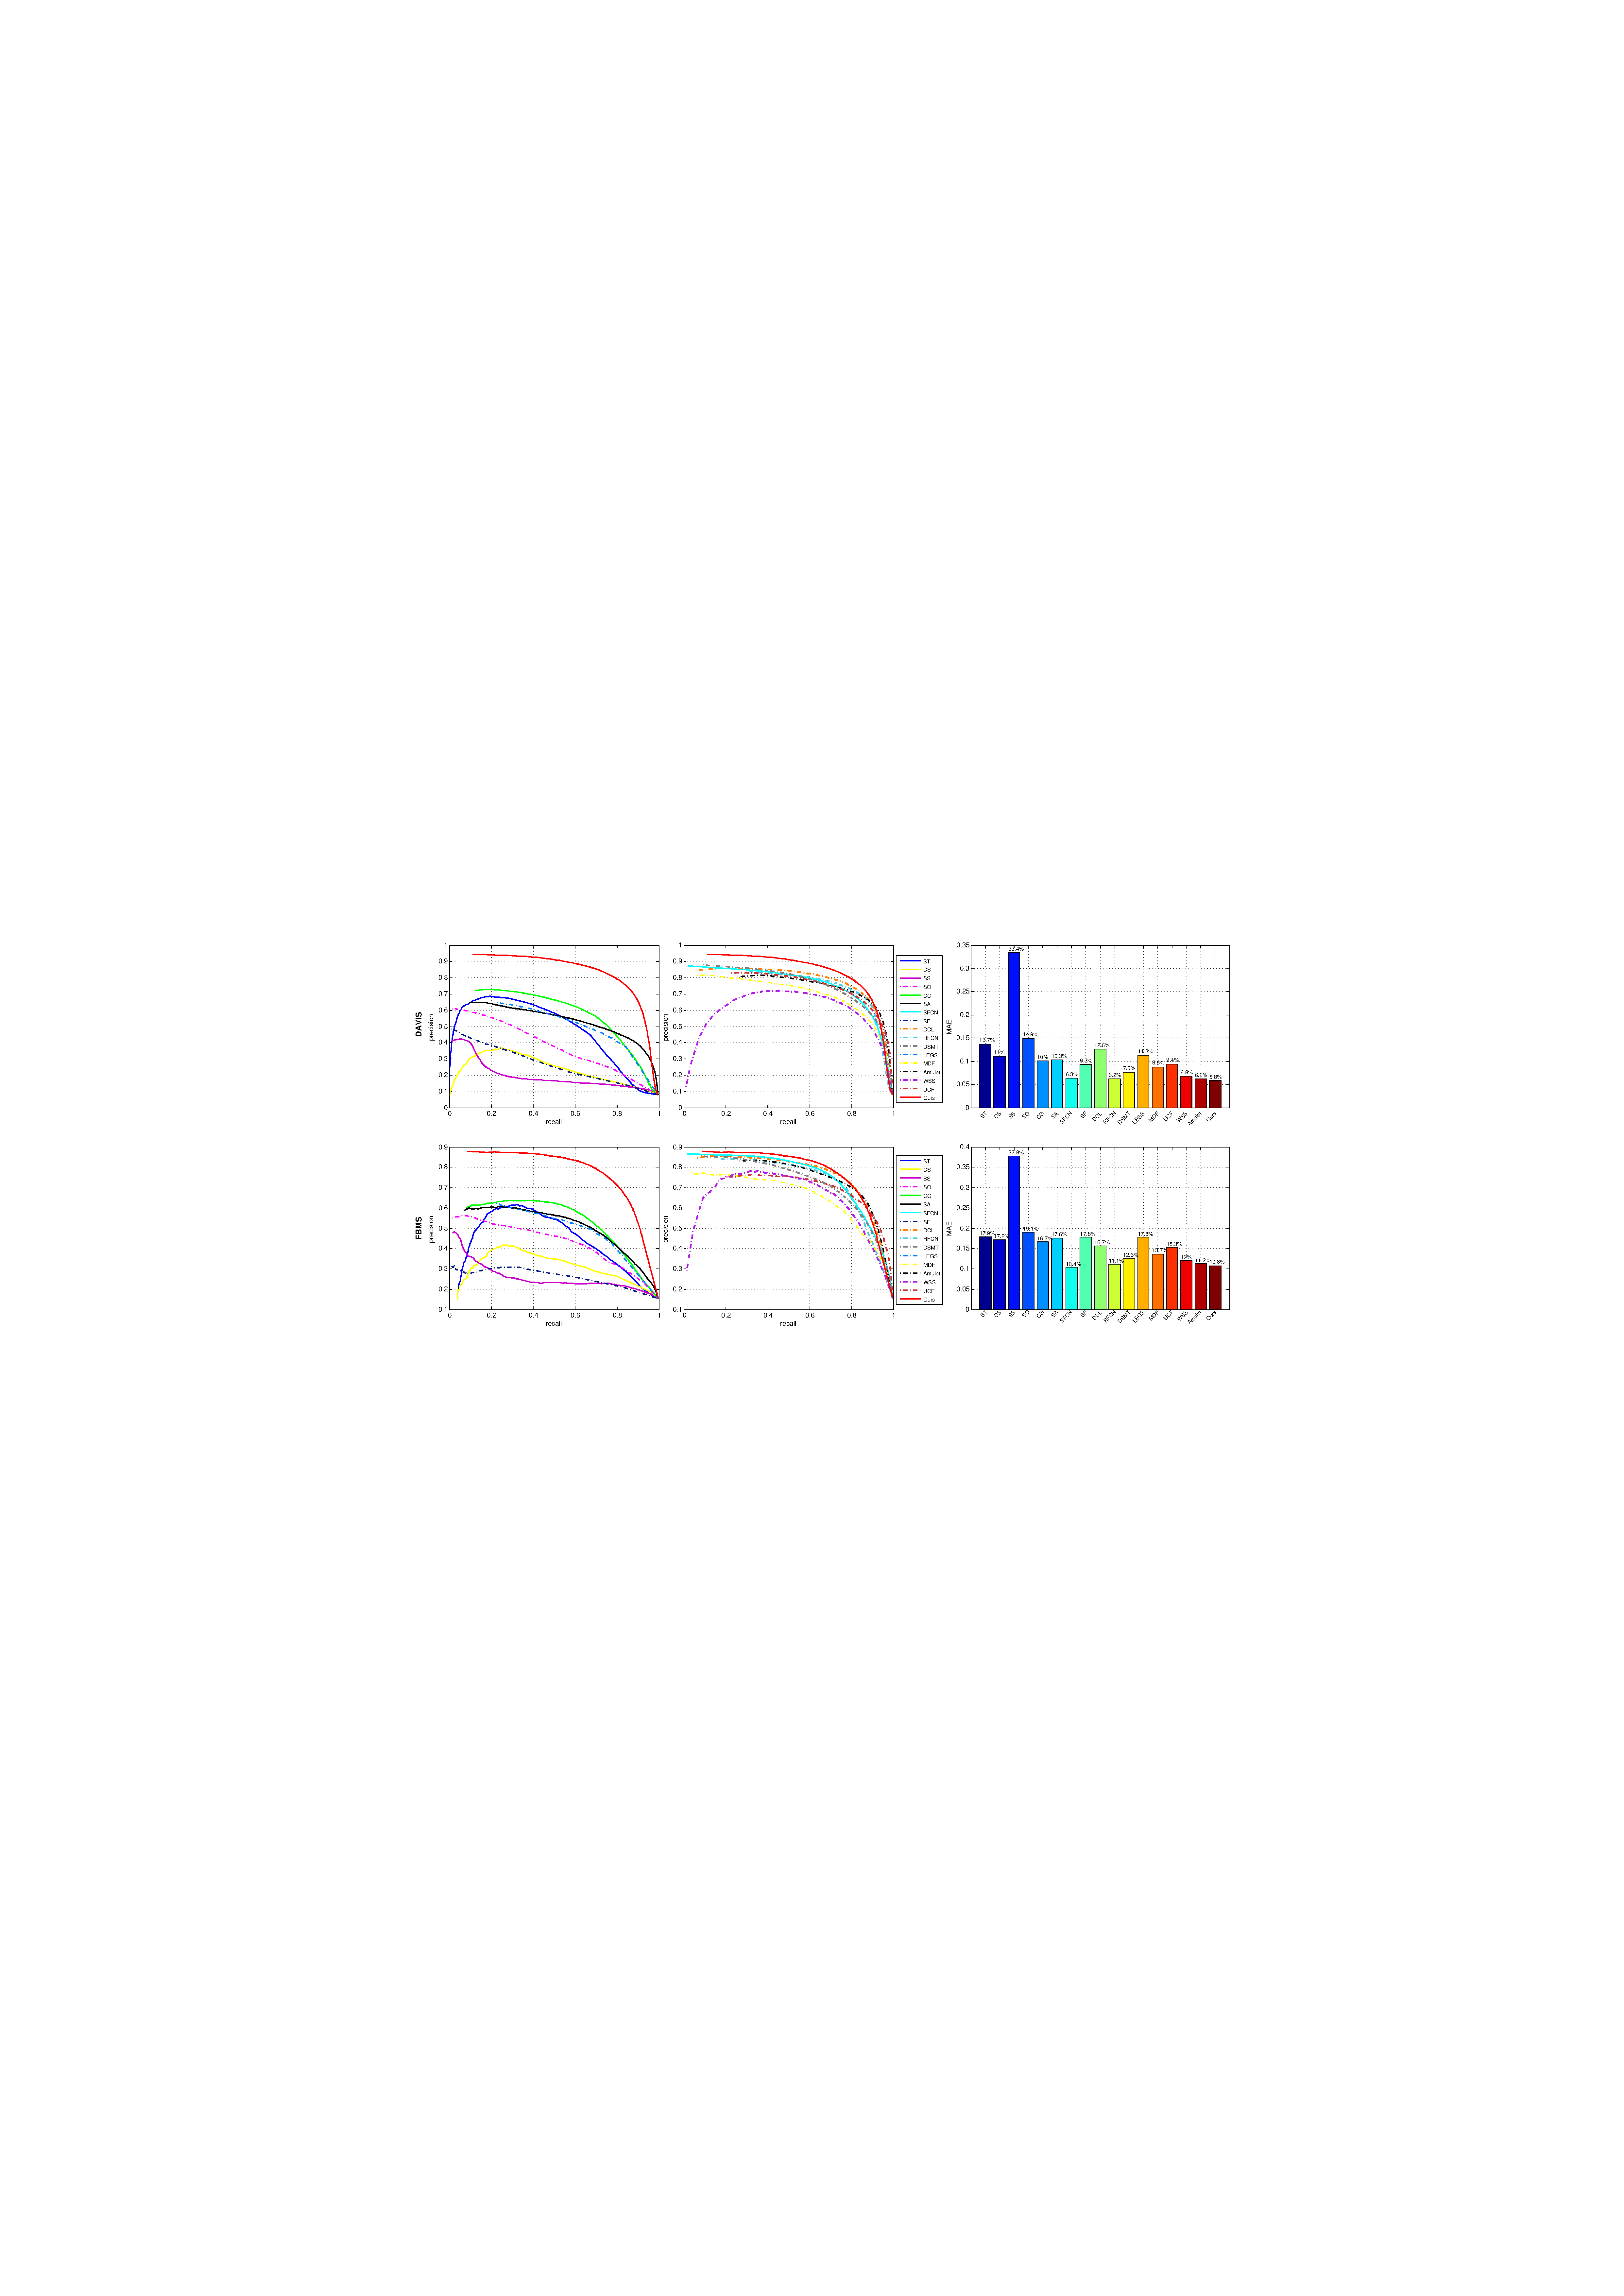
\includegraphics[width=15cm]{figures/methos_compare_new2}
\caption{SCNN比较16个不同的显著性检测方法,其中包含6个视频显著性方法(实线)和10个图像显著性检测方法(虚线)。DAVIS的PR曲线和MAE柱状图在上,FBMS的曲线与柱状图在下}
\label{figure4}
\end{figure*}

上述的所有模型再加上本文提出的SCNN模型,共19个,其PR曲线和MAE柱状图一起展示在图\ref{figure4}中。可以清楚地看到,本文提出的SCNN模型在PR曲线和MAE上都取得了显著的提升。在DAVIS数据上,SCNN的PR曲线明显地超过的其他的方法,而在FBMS数据集上,SCNN也有不小的提升。在MAE方面,SCNN把其数值在DAVIS和FBMS数据上分别下降到的5.8\%和10.8\%。

\begin{figure}[tbp]
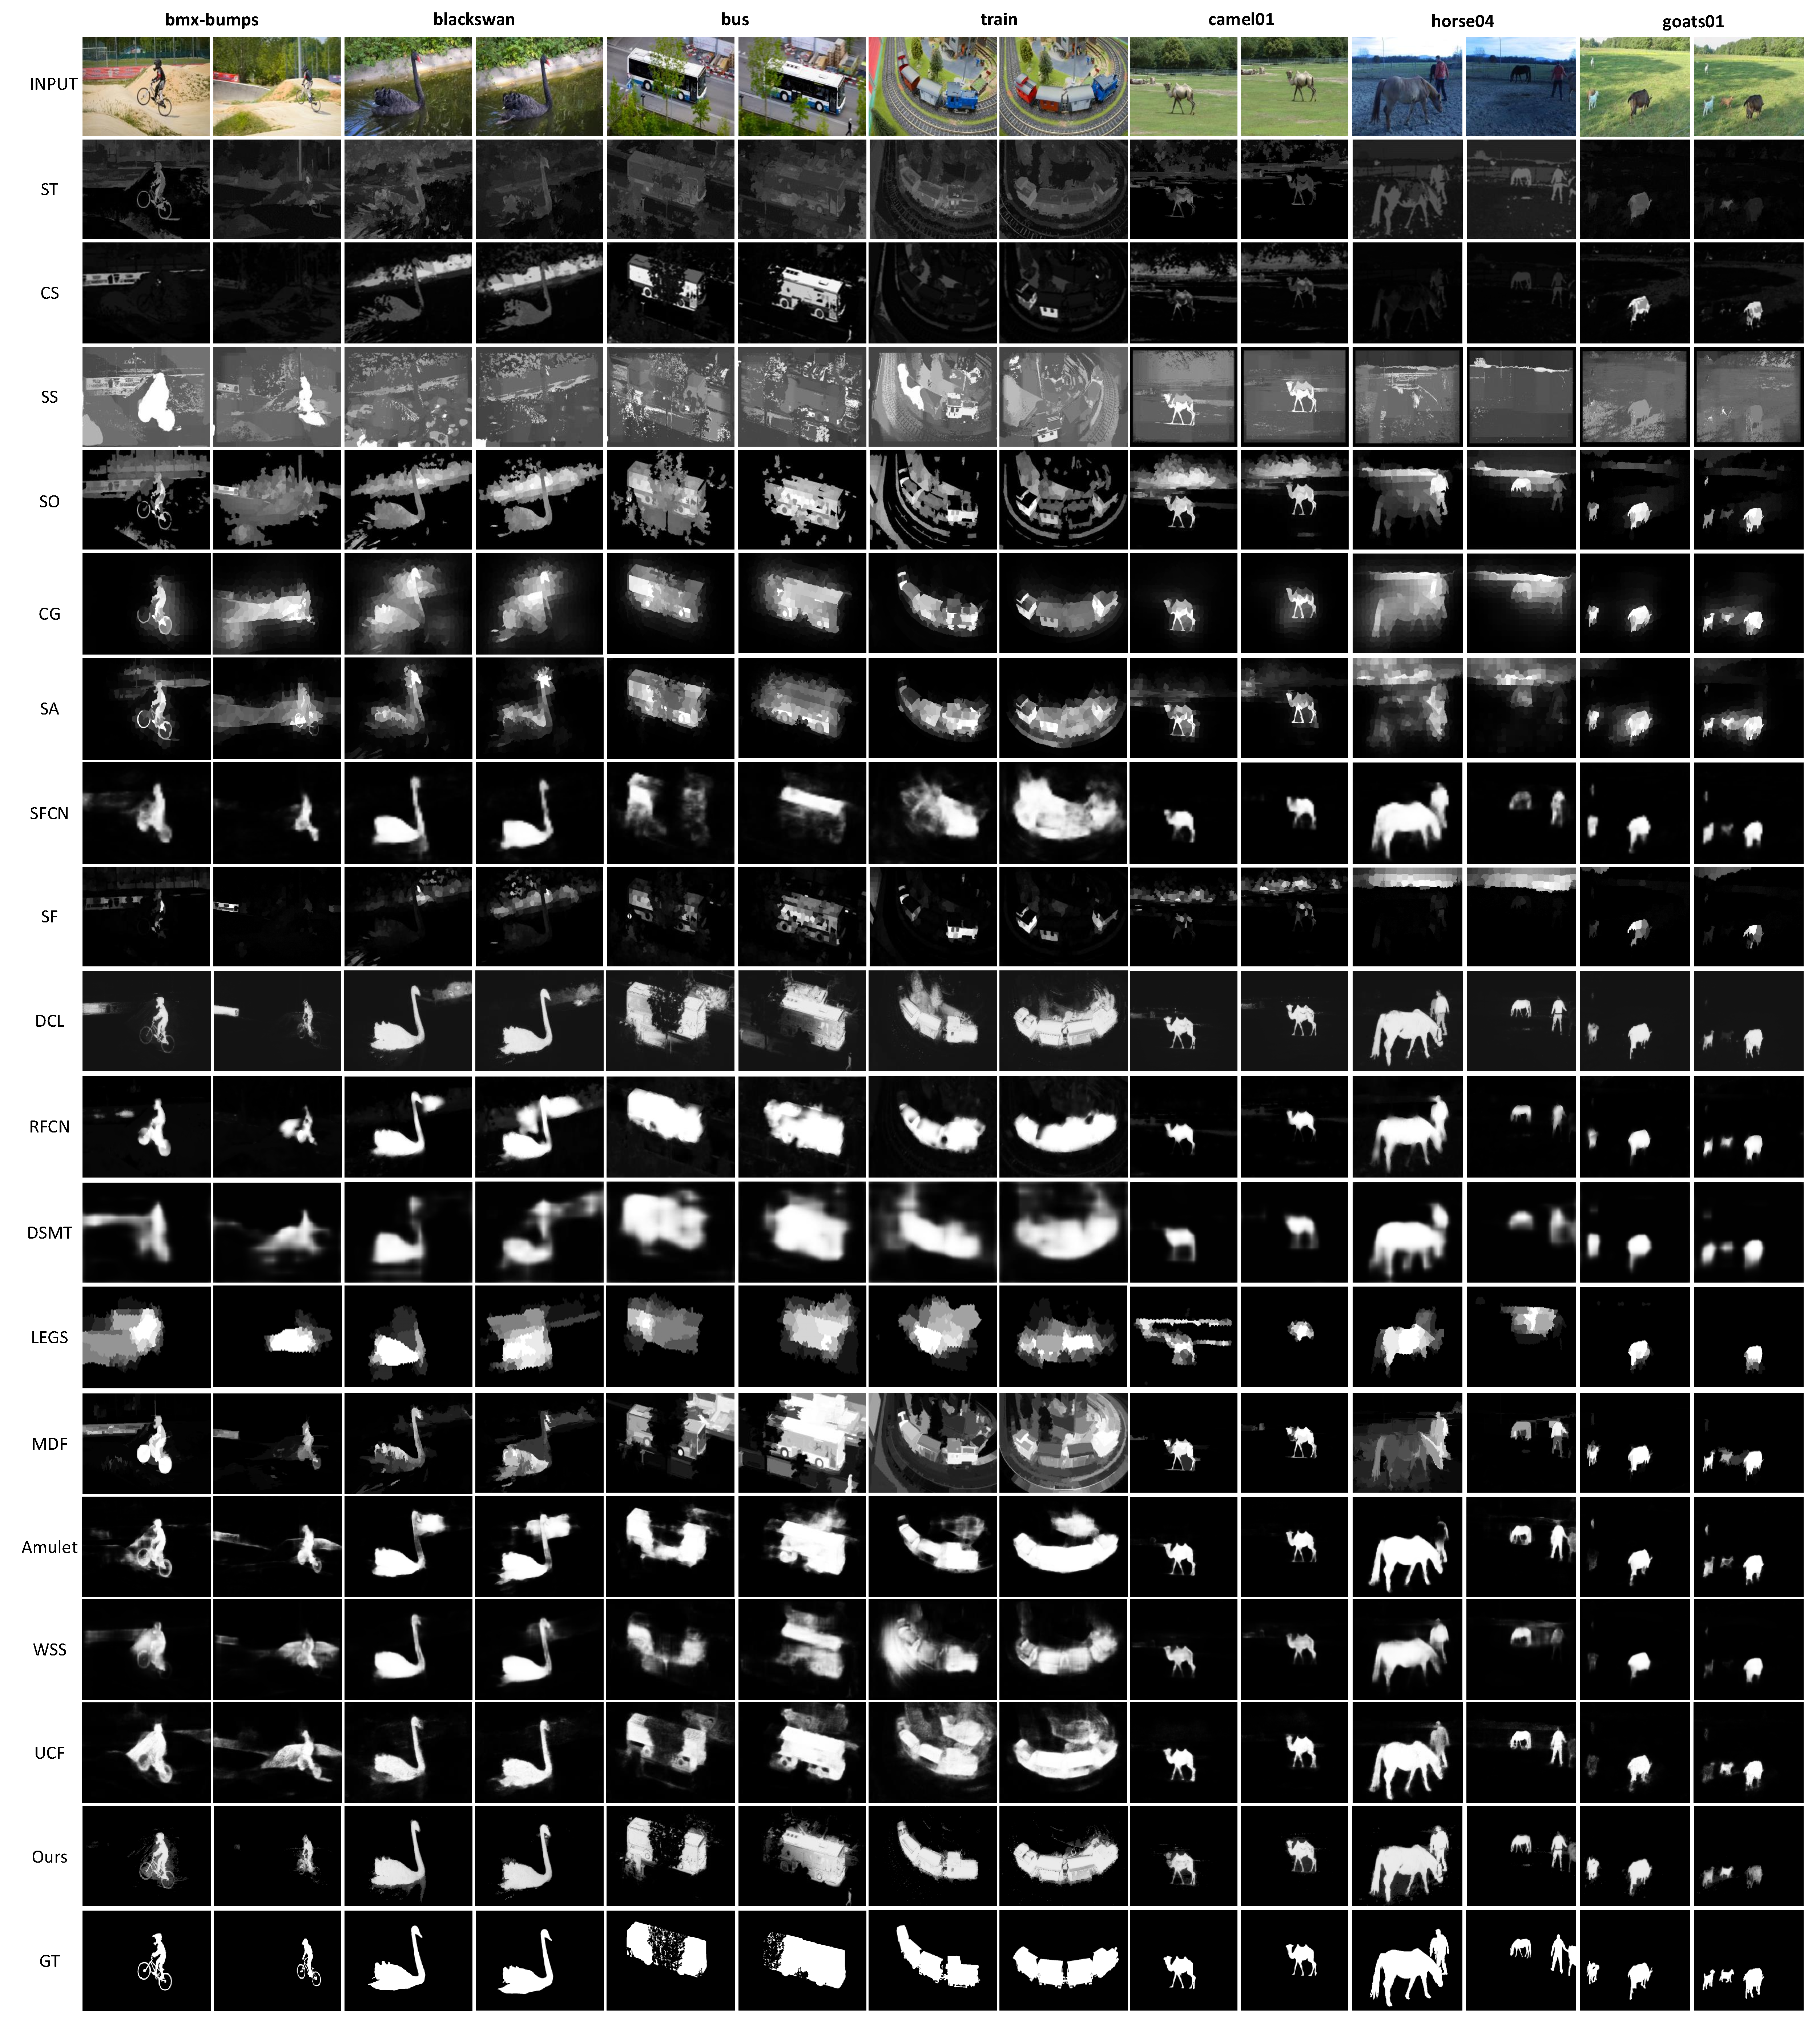
\includegraphics[width=15cm]{figures/show_new}
\caption{部分的显著图展示,其中bmx-bumps、 blackswan、 bus和train序列是来自DAVIS数据集,camel01、 horses04和goats01是来自FBMS数据集。从品质上来看,SCNN生成的显著图可以移除静态显著区域的干扰并生成与真值最为相近的显著图}
\label{figure5}
\end{figure}

图\ref{figure4}是SCNN的定量分析,而在图\ref{figure5}则是SCNN的定性分析,展示的是SCNN在DAVIS和FBMS中视频序列中生成的显著图。前面四个序列(bmx-bumps、 blackswan、 bus、 train)是属于DAVIS数据集,后三个(camel01、horse04、goats01)则属于FBMS数据集。如果所示,SA和CG是采用运动轨迹建模的方法,其生成的显著图甚至不如图像显著检测的方法(如DCL、 RFCN、 MDF)。基于深度学习的方法在可以在视频序列中成功地检测出大多数显著区域,但是它们也同时会高亮一些背景区域。例如,序列bmx-bumps的红色广告牌和序列blackswan的河岸都是判别为显著性区域而被高亮的背景噪声。造成这些噪声的原因主要是缺少运动信息,而本文提出的SCNN恰恰引入了鲁棒性高的时空先验来引导网络学习。因此,本文的方法可以有效地去除非运动显著区域的干扰并生成高质量的显著检测图。于此同时,SCNN对多显著目标的检测也就好的结果,例如在horse04和goats01序列中,所有的马和羊都被SCNN检测到,而其他的方法只能检测出部分目标。

\begin{figure}[tbp]
\center
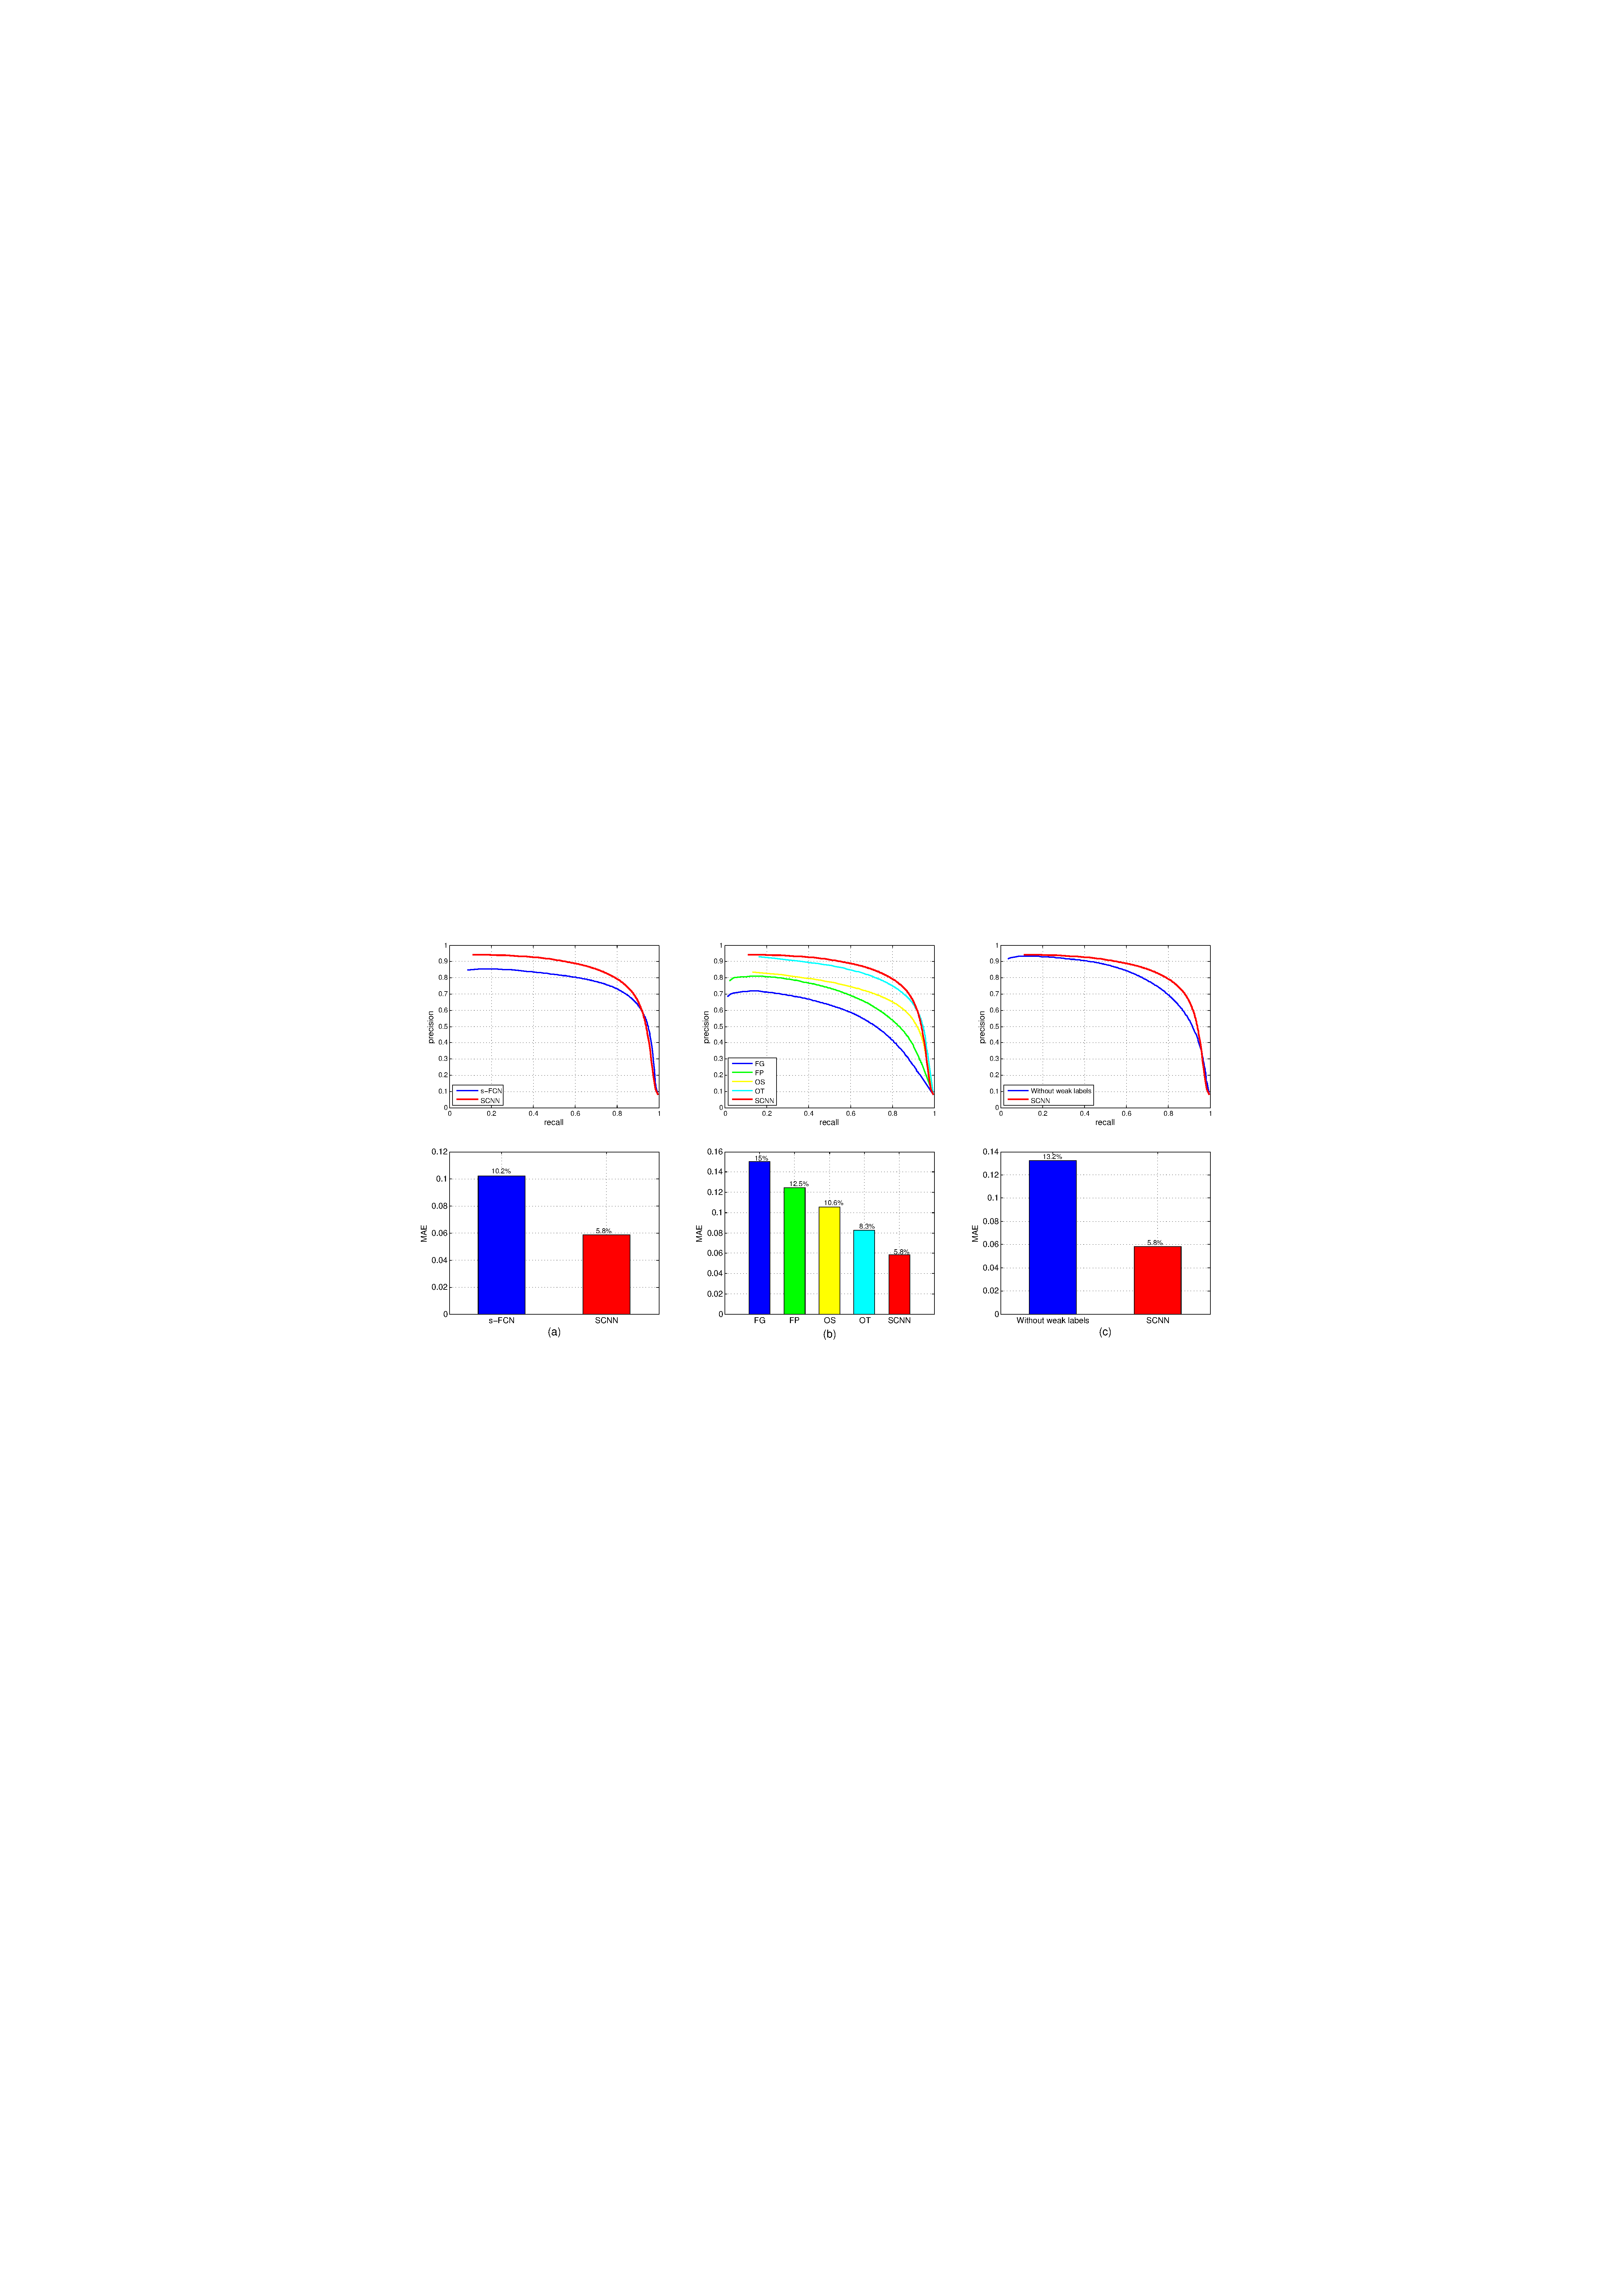
\includegraphics[width=15cm]{figures/self_compare3}
\caption{由不同配置在DAVIS数据上生成的PR曲线与MAE柱状图。(a)单全卷积模型和SCNN级联模型的比较。(b)不同静态与动态先验组合的比较。(c)并行弱监督迭代策略的验证}
\label{figure6}
\end{figure}

\subsection{各个子模块的有效性验证}

为了验证SCNN各个模块的有效性,本文利用DAVIS数据集针对级联网络结构、时空先验和弱监督方法的有效性做了实验验证。

首先,为了验证级联网络的有效性,设计了一个单全卷积结构的网络(s-FCN)。其结构与SCNN中的静态子网完全相同,只使用视频帧训练网络,没有运动先验的引导。实现结果如图\ref{figure6}中的(a)所示,SCNN的PR曲线明显的比单全卷积结构高。在MAE方面,单全卷积结构有10.2\%,而SCNN可以低至5.8\%,这两个结果表明相比于单全卷积结构,本文提出的级联结构SCNN可以提升很多,再加入时空先验之后,SCNN的结构合理,可以很好的利用先验引导学习显著特征。

其次,为了验证时空先验的有效性,而且探求还是的验证组合,本文尝试了不同先验组合。为了保持实验公平性,这次验证实验除了先验组合外,其他结构保持不变。所以的先验组合如下:
\begin{itemize}
\item \textit{FG}:在这一个设计中,三通道的光流图直接转化为单通道的灰度图。然后该灰度图像与SCNN中第一个全卷积子网产生静态先验$P_s$,还是视频帧利用公式 \ref{eq3_1})组合一个五通道的输入,并用于引导SCNN的第二全卷积网络。
\item \textit{FP}: 由公式\ref{eq3_2}产生的运动先验$P_t$和FCN产生的静态先验 $P_s$,再加上视频帧组合成一个五通道的图像作为SCNN的输入。
\item \textit{OS}: 只使用静态先验$P_s$与视频帧组成四通道的网络输入来进行网络学习。
\item \textit{OT}: 只使用运动先验 $P_t$与视频帧组成四通道的网络输入来进行网络学习。
\end{itemize}

\begin{figure}[tbp]
\center
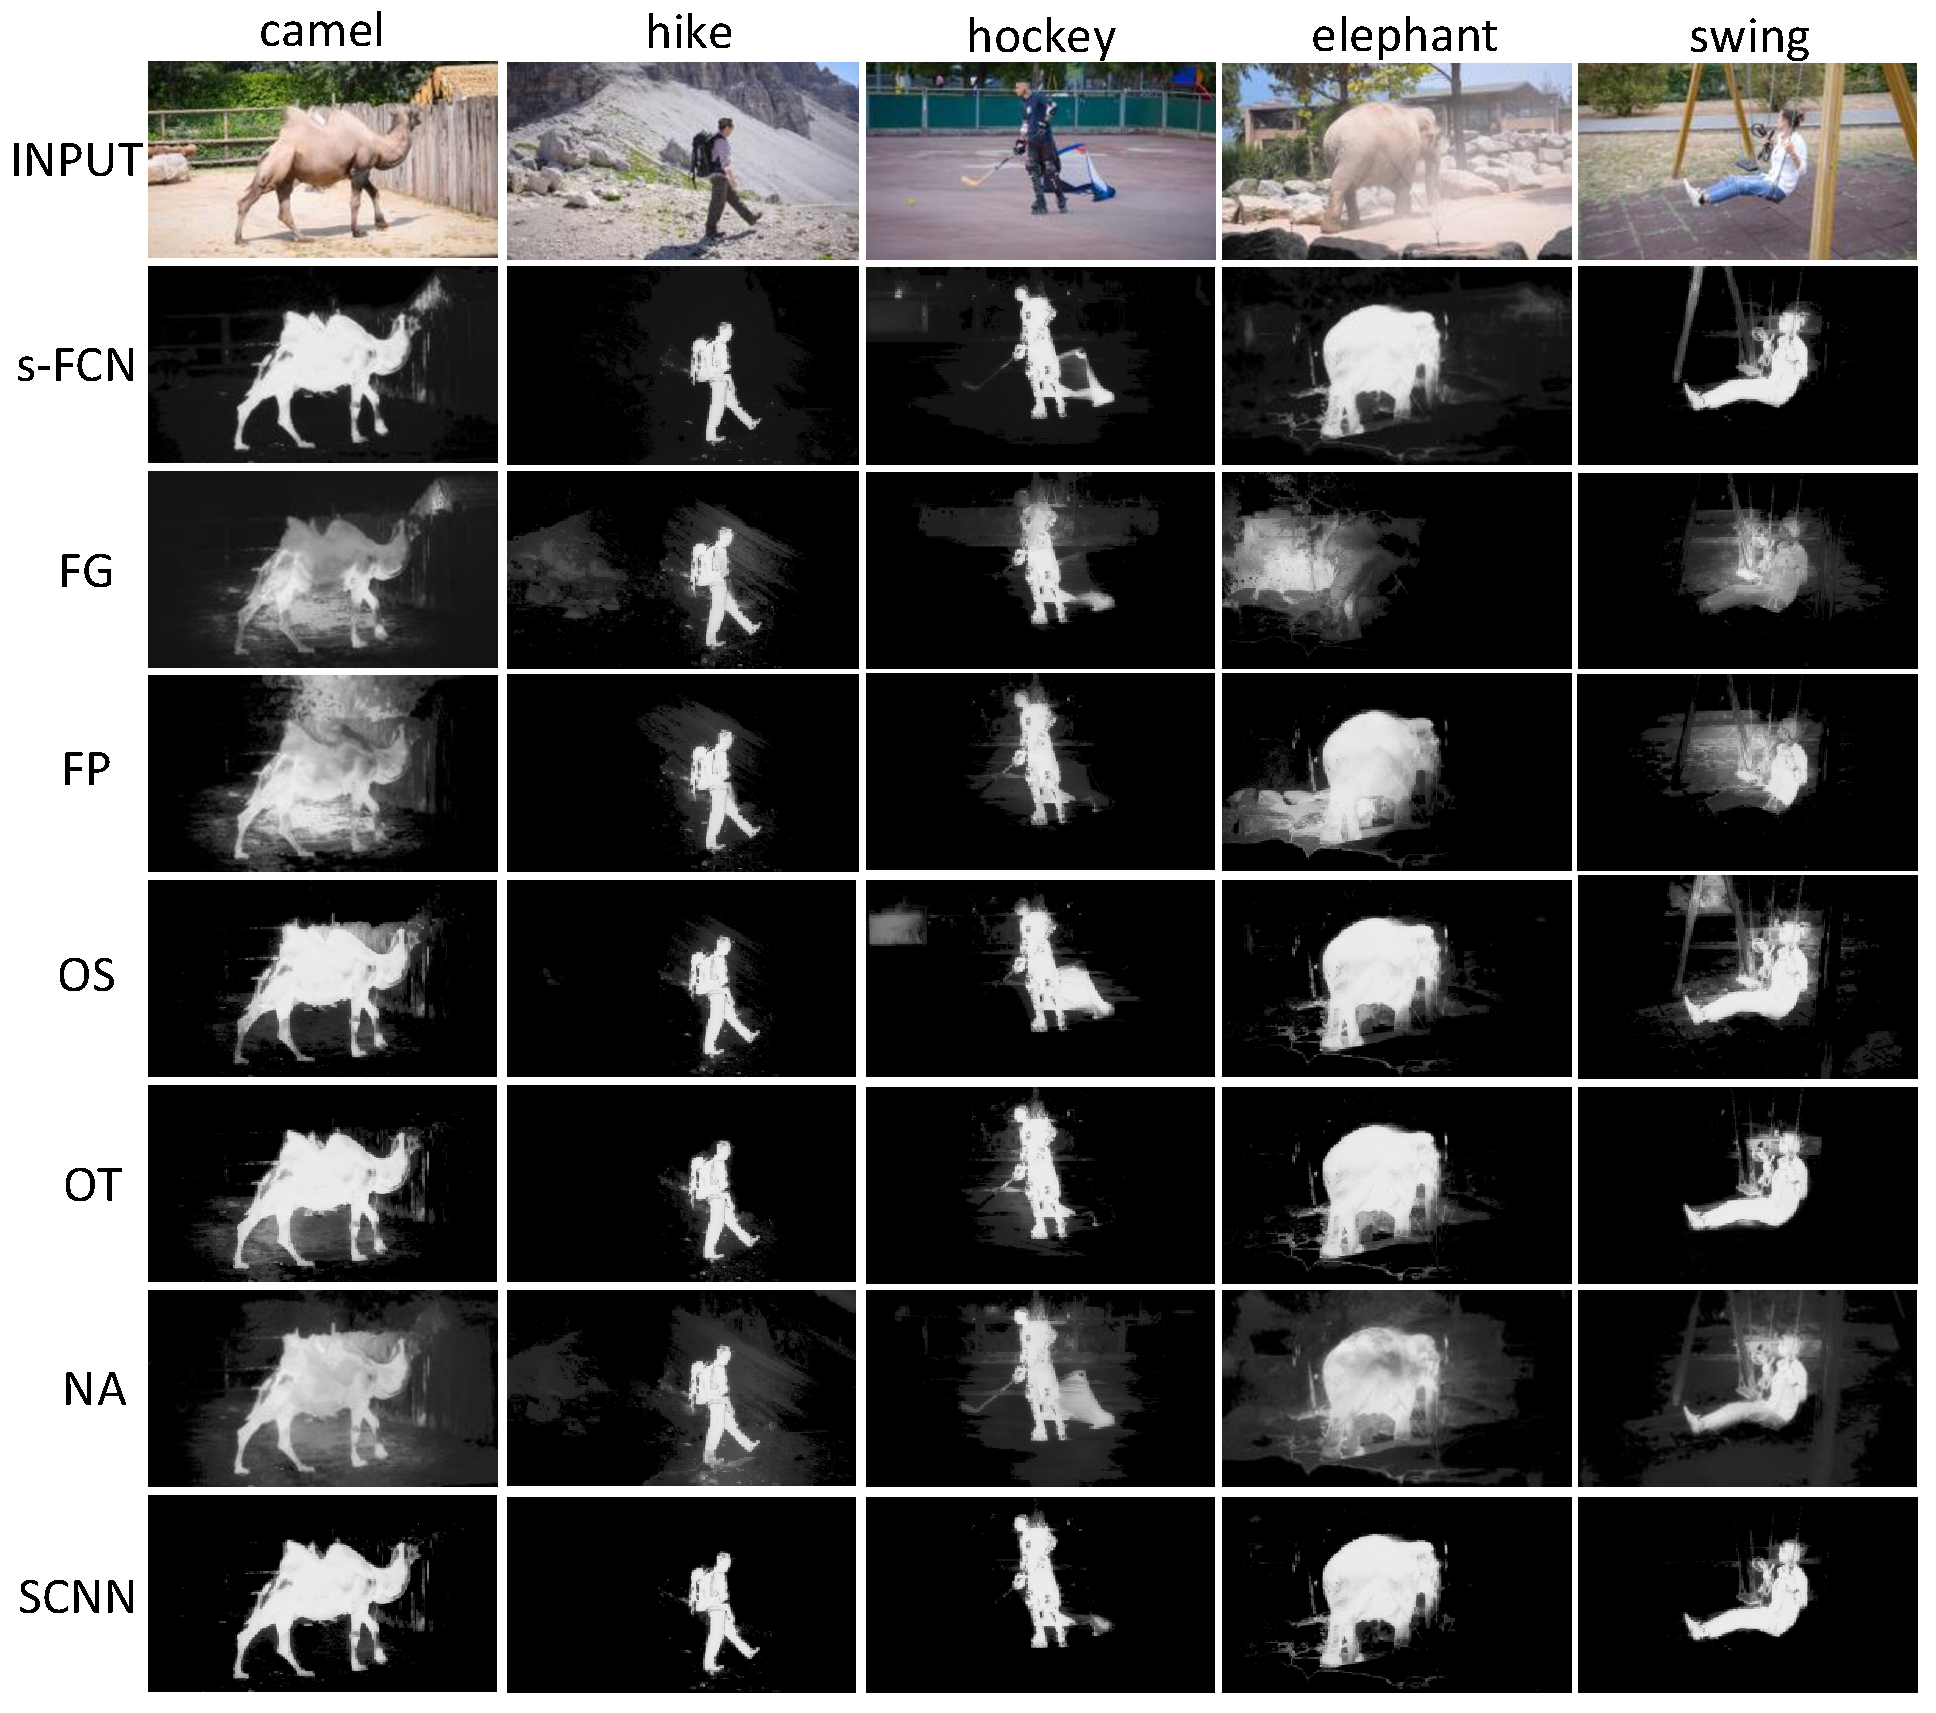
\includegraphics[width=10cm]{figures/show2}
\caption{不同配置生成的显著图。从上到下分别为单卷积网络(s-FCN)、组合灰度光流先验和静态先验(FG)、组成静态先验与动态先验为五通道输入(FP)、只使用静态先验(OS)、只使用动态先验(OT)、不使用并且弱监督迭代训练策略(NA)与最终SCNN模型。}
\label{figure10}
\end{figure}

如图\ref{figure6}中的(b)的实验结果,我们可以清晰地看到本文提出的使用对应像素相乘的方法最为合理,相比于其他四种的组合都有不少提高。在一些复杂的场景上,静态先验会存在不少背景噪声,而且这些噪声会直接影响SCNN第二个全卷积子网的学习。对应像素相乘的引入,可以很好的移除这些背景噪声。其次,可以增强两个先验的共同区域,使得SCNN生成的显著图可以很好地保留主体显著区域。通过,这一个验证实验可以证明本文提出的时空先验和融合先验的策略都是切实可行且有效的。

在训练网络时,SCNN引入了一个并行弱监督迭代的训练策略,从而在训练过程中产生大量的弱标签来辅助网络学习。为了验证这一个训练策略的有效性,本文也设计了一个对比实验,分别采用和不采用弱监督训练策略来进行网络优化。实验的结果如图\ref{figure6}(c)所示,可以清楚地看到,在使用本文提出的并行弱监督迭代策略后,SCNN生成的显著图有明显提高,PR曲线与MAE柱状图都有不小的提升。同时,图\ref{figure10}也展示了各种网络配置生成的显著图,可见SCNN的各个模块都是有效的,缺少任一个模型都会使生成的显著图造成不小的影响。

\begin{figure}[tbp]
\center
\subfigure[比较使用稠密条件随机场的使用]{
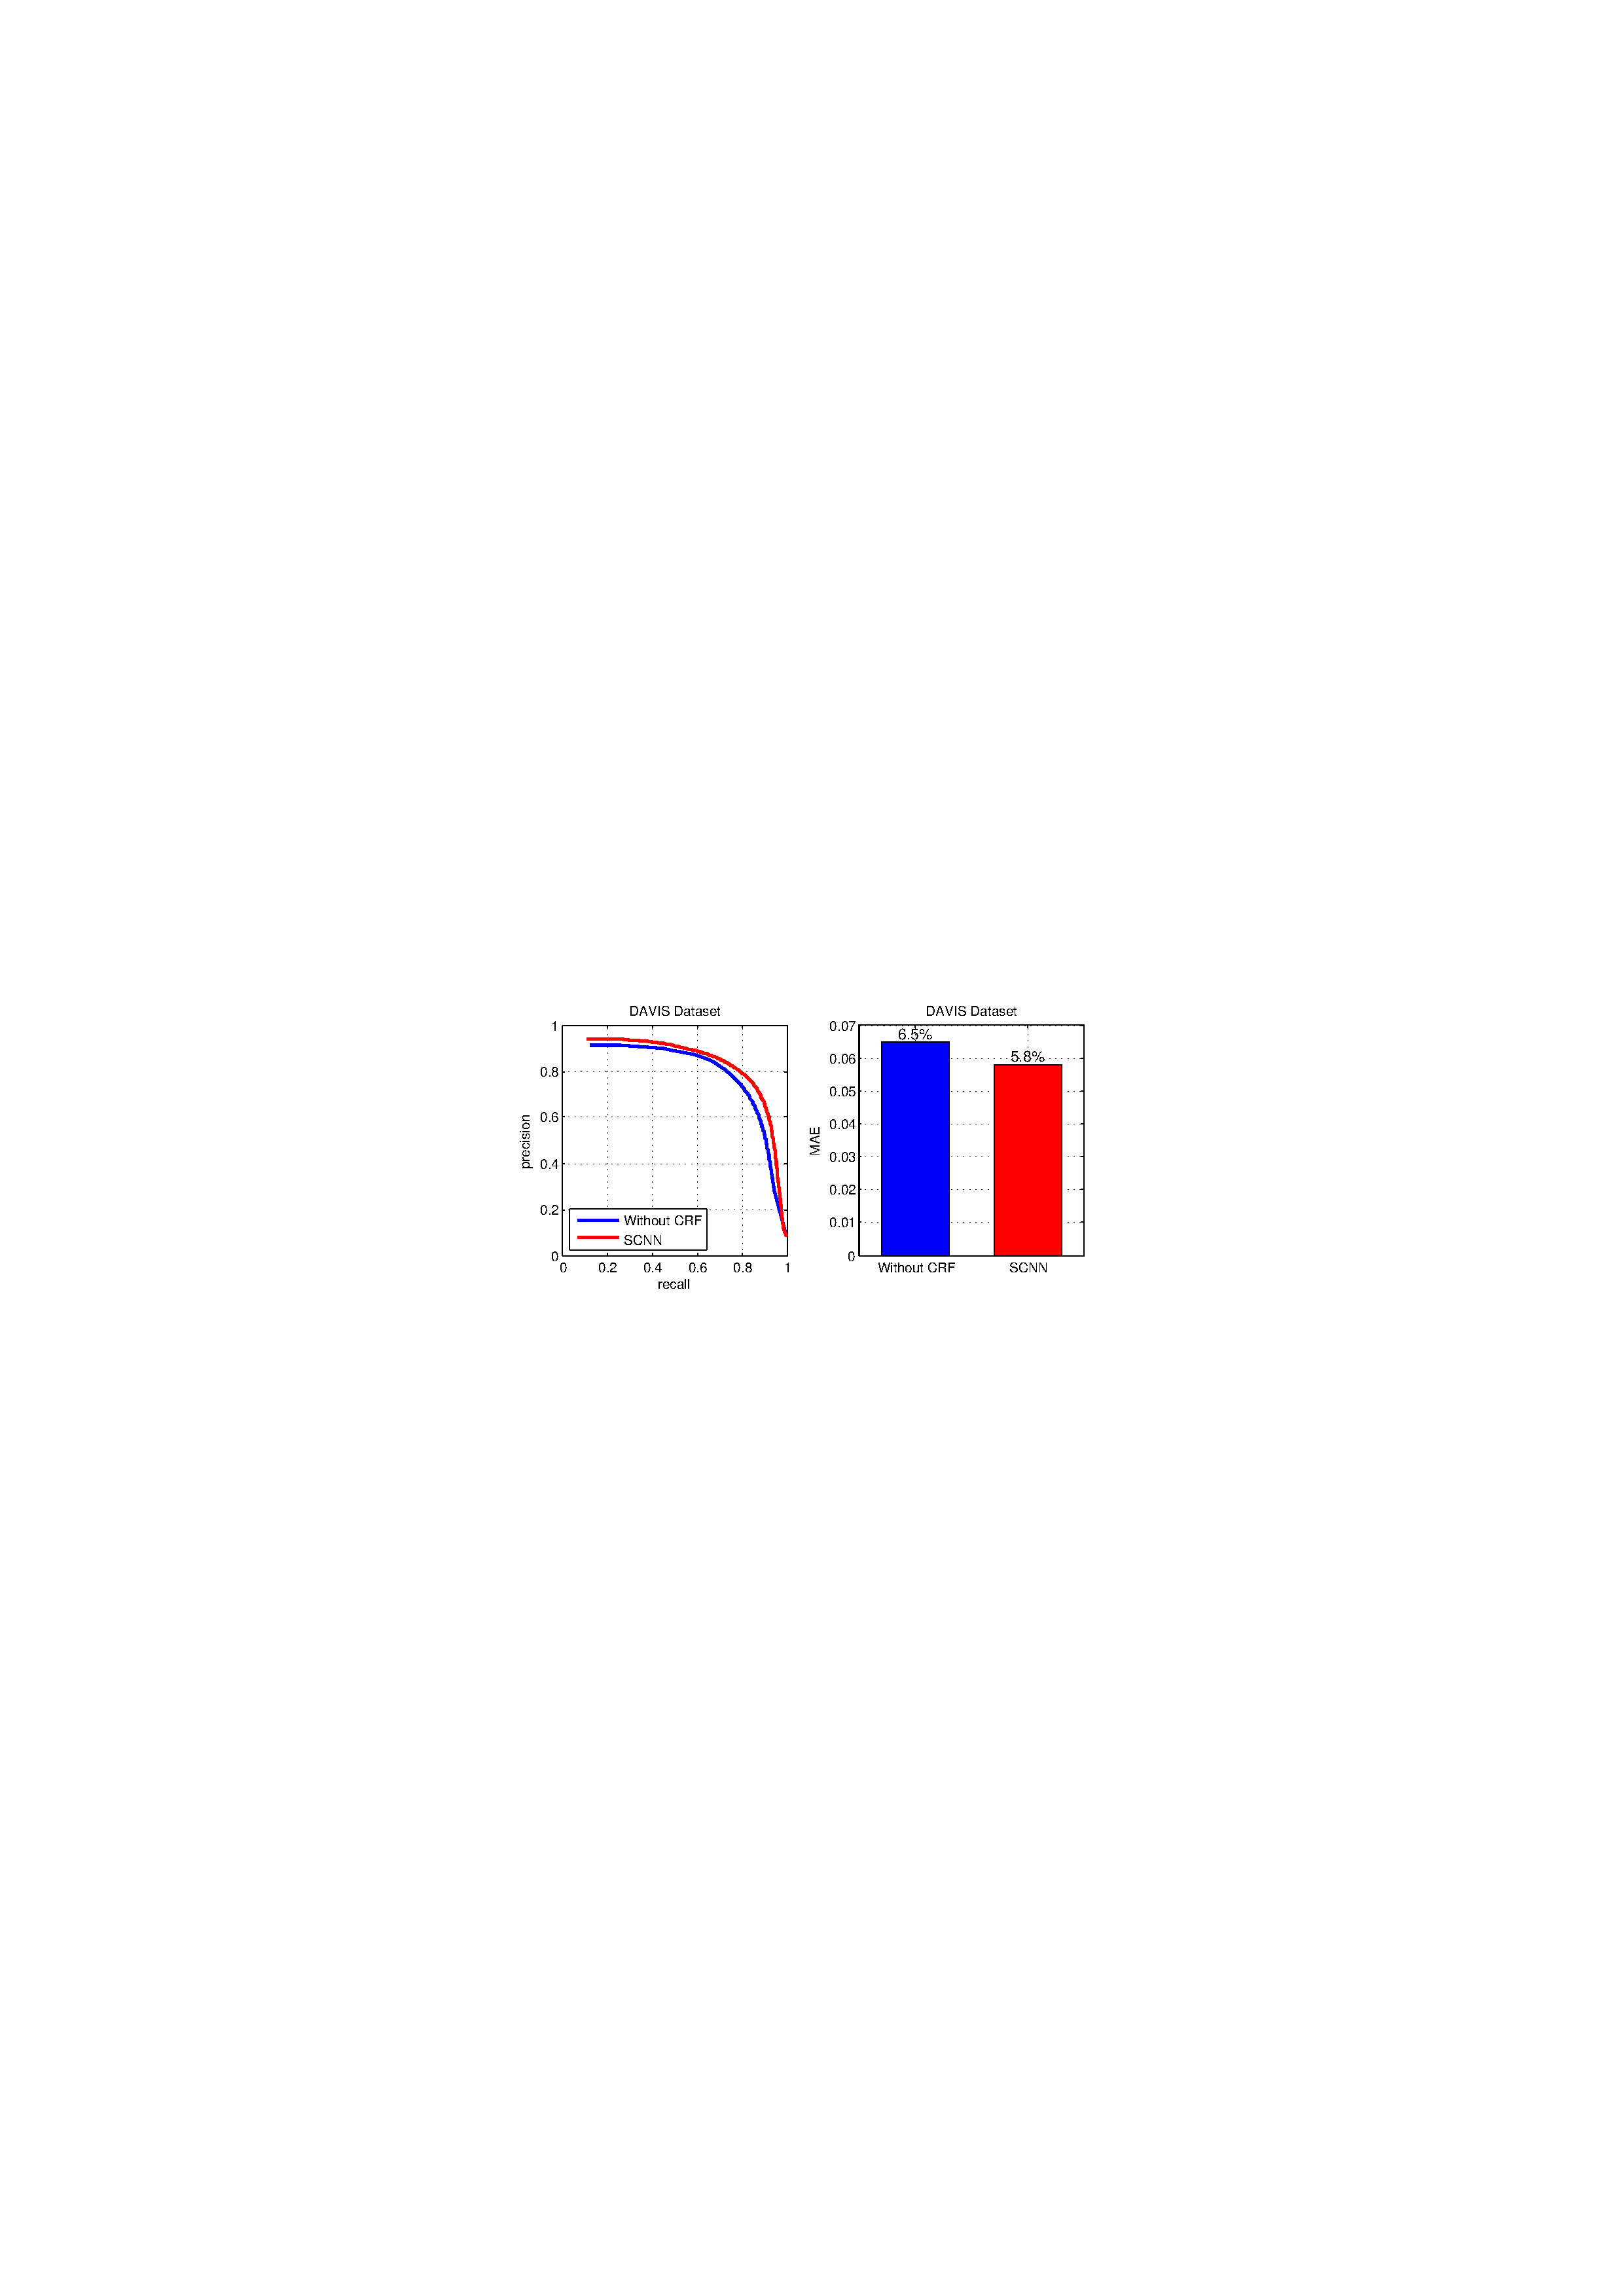
\includegraphics[width=8.5cm]{figures/postprocessing2}
}
\subfigure[比较多尺度特征图的使用]{
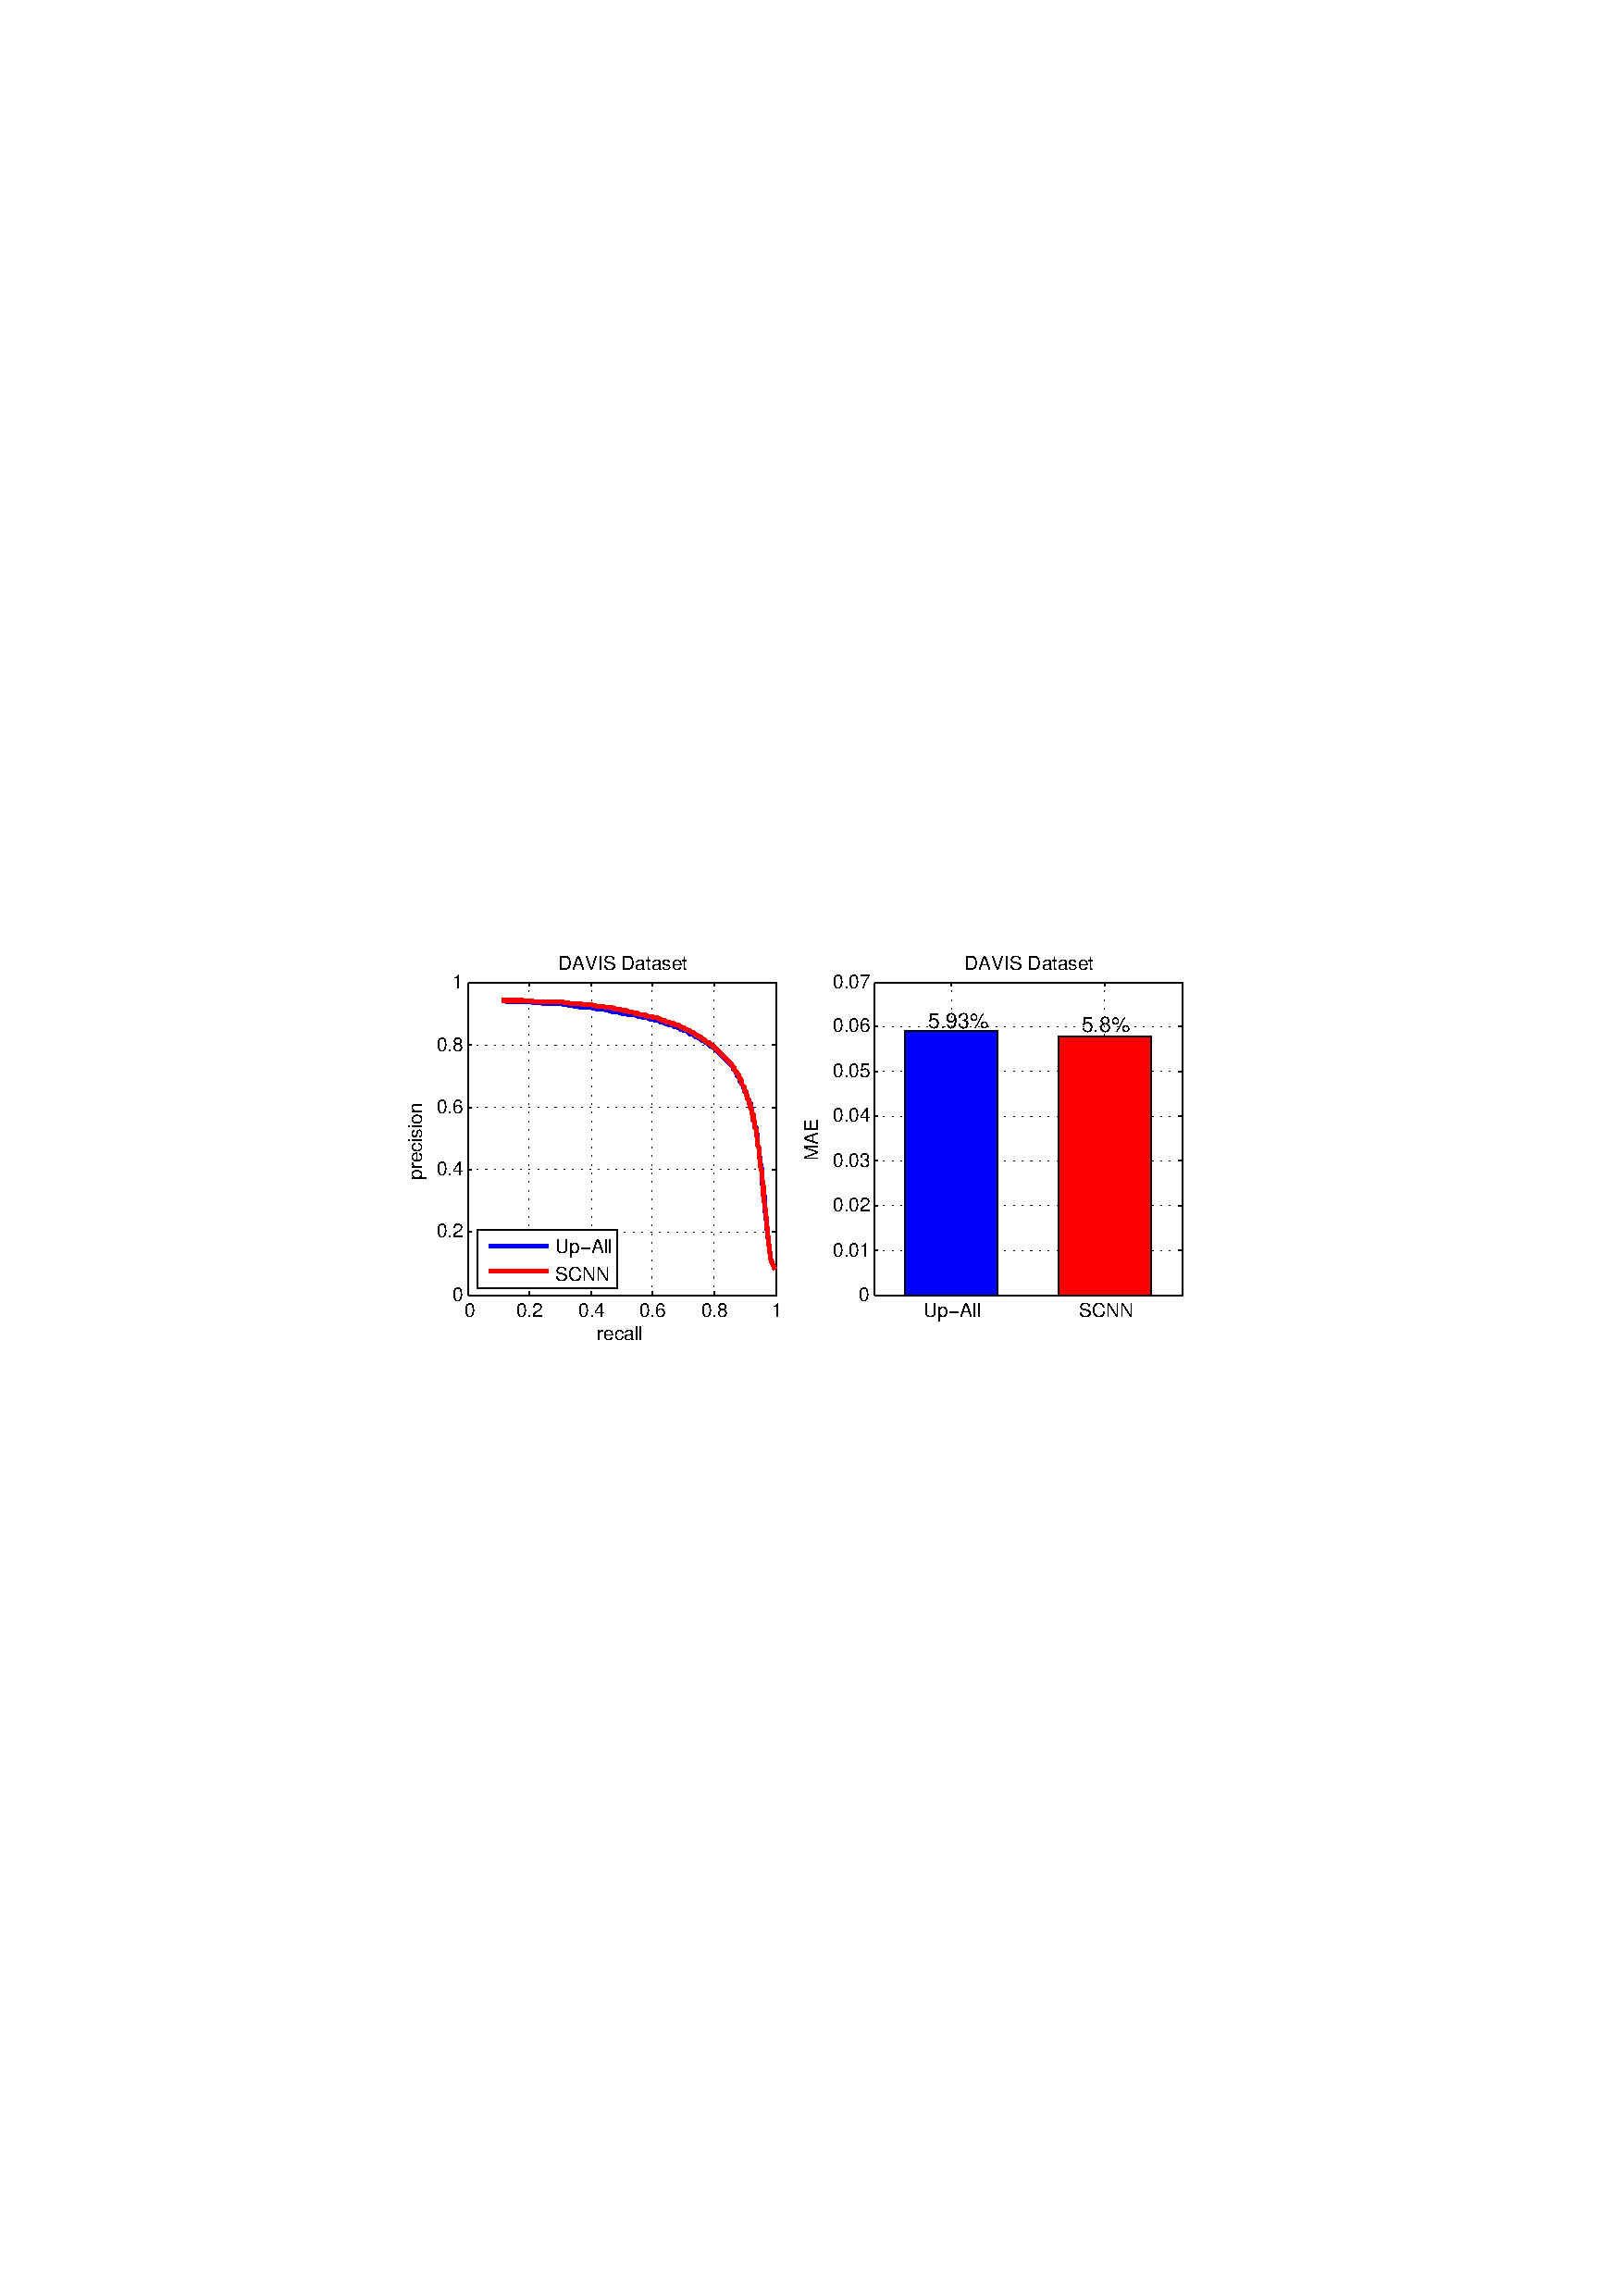
\includegraphics[width=8.5cm]{figures/pool_test}
}
\caption{稠密条件随机场和多尺度特征的实验验证}
\label{diff_config}
\end{figure}

在本文提出的SCNN中,为了更好精炼显著图,稠密条件随机场的方法(Dense CRF)被引入,作为显著图的后处理方法。并且,在SCNN模型上,多尺度的特征图也被用来提升显著图质量,但是在使用多尺度特征图时也不是所有的特征都对最终的显著图有促进作用。在此,本文设计了两个实验分别验证稠密条件随机场和多尺度特征的有效地。如图\ref{diff_config}所示,其中图(a)是使用Dense CRF与否的比较,可看到Dense CRF对全局的显著图有明显的提升效果。而图(b)则是多尺度特征图的验证,蓝色的曲线和柱状图为使用全部尺度的特征,即VGGNet每一个卷积块后都设计一个上采样的模块,共6个,在网络的末端再求和获得最终的显著图。本文则发现在视频显著性检测任务中,多尺度的特征图不是越多越好,最后通过此实验验证得到只使用最后两个卷积块的上采样特征图进行融合,其效果为图(b)中的红色曲线和柱状图。由此可见,在视频显著性检测领域,神经网络的高层语义特征比底层特征更重要,利用其生成的特征图也更好。

\begin{table}[htbp]
\centering
\caption{各方法在DAVIS数据上的平均运行时间(秒每帧)}
\renewcommand{\arraystretch}{1.2}
%\begin{tabular}{|l|p{0.8cm}|p{0.95cm}|p{1.0cm}|p{1.05cm}|p{0.99cm}|}
\begin{tabular}{|c|c|c|c|c|c|c|}
\hline
\hline
Method &SCNN  &SCNN$_f$ &ST  &CS        &SS  &SO  \\
\hline
Time(s) &38.511 &2.53 &28.193 &1.175   &37.176 &0.671 \\
\hline
\hline
Method   &CG   &SA     &DLVS  &SF   &DCL    &RFCN        \\
\hline
Time(s)  &38.075  &38.751  &0.473 &0.842 &0.670   &4.580         \\
\hline
\hline
Method        &DSMT   &LEGS &MDF   &Amulet   &UCF  &WSS\\
\hline
Time(s)       &0.14     &0.206  &11.33 &5.299   &0.151 &0.024\\
\hline
\end{tabular}
\label{table2}
\end{table}

\begin{table}[htbp]
\centering
\caption{本章提出方法在各个模块上消耗的平均时间(秒每帧)}
\renewcommand{\arraystretch}{1.2}
\begin{tabular}{ |l|l|r|r| }
%\hline
%\multicolumn{3}{ |c| }{Time sheet} \\
%\hline
\hline
\hline
Model & Component & Time (s) & Ratio (\%)\\ \hline
\multirow{5}{*}{SCNN} & Optical flow computation & 36.720 & 95.36\\
 & Temporal prior generation & 0.823 & 2.14\\
 & Neural network processing & 0.685 & 1.78\\
 & Saliency refinement & 0.283 & 0.72\\\cline{2-4}
 & Total & 38.511 & 100\\ \hline
\hline
\multirow{5}{*}{SCNN$_f$} & Optical flow computation & 0.739 & 29.2\\
 & Temporal prior generation & 0.823 & 32.5\\
 & Neural network processing & 0.685 & 27.1\\
 & Saliency refinement & 0.283 & 11.2\\\cline{2-4}
 & Total & 2.53 & 100\\ \hline

\end{tabular}
\label{table3}
\end{table}

\subsection{时间效率分析}

SCNN方法的所有实验都在一个GPU工作站上运行,其配置是一个Intel(R) i7-5820 CPU (3.3GHz)、一个Nvidia Geforce TITAN X GPU显卡(12 GB memory)和64G内存。表\ref{table2}展示的是在DAVIS数据集中,所有方法的处理一帧视频需要花的时间。在所有方法中,CG、SA、SS和本文提出的SCNN使用到了光流,由于光流提取比较耗时,所以处理时间相对较慢。而表中的SCNN$_f$则引入FlowNet2.0 \cite{8099662}来提取光流。由于FlowNet2.0是基于深度模型的方法,其相比于传统提取光流的方法\cite{Sun2014A},减小了很多像素级的运用,从而大大地加快的光流提取速度。表\ref{table3}则展示了SCNN和SCNN$_f$每一个模块消耗的平均时间。从表中,我们可以看到FlowNet2.0可以把光流提取时间从36.720s下降到0.739s,进而把SCNN的运行速度从38.511s降至2.53s.

\section{小结}

在此章内容中,本文提出一个新颖的级联神经网络SCNN来进行视频显著性检测。这一方法整合了帧内的静态先验和基于光流的先验,并通过融合后的时空先验引导网络学习,从而使得网络可以很好地消除非运动目标的噪声影响并生成高质量的显著图。本文巧妙地运用光流图分割得到几乎完成的显著运动目标,同时运用超像素的深度特征可以得到较为准确的运动先验,这一个先验可以很好地引导SCNN,从而学习到鲁棒的运动特征。针对视频显著性像素级标签少且不连续的问题,本文又提出了并行弱监督迭代的策略来训练神经网络,很好地解决了训练数据不足的问题。本文在通用数据集DAVIS与FBMS中的实验(PR和MAE的评价标准)可以证明SCNN是优于其他图像和视频的最新方法。